\documentclass[onecolumn]{IEEEtran}

% Basic required LaTeX packages
\usepackage[english]{babel} 
\usepackage[utf8]{inputenc} 
\usepackage[T1]{fontenc}

% Packages which allow format customisation
\usepackage{titling}
\usepackage{cite}
\usepackage{caption}
\usepackage{textcomp}
\usepackage{xcolor}
\usepackage{etoolbox} 
\patchcmd{\section}{\centering}{}{}{} % uses the etoolbox package to left align section headings
\usepackage{indentfirst}
\usepackage{subcaption}

% Packages which help display things like maths and images correctly
\usepackage{amsmath,amssymb,amsfonts}
\usepackage{algorithmic}
\usepackage{graphicx}
\usepackage{hyperref}

% No line indent in subsubsection %
\makeatletter
\def\subsubsection{\@startsection{subsubsection}{3}{\z@}{0ex plus 0.1ex minus 0.1ex}{0ex}{\normalfont\normalsize\itshape}}
\makeatother

%% START DOCUMENT %%
\begin{document}

%% TITLE %%
\title{Smart Home Adapters -- Technical Report}
\author{Group 18 -- HalsPals}
\date{10/04/19} 
\maketitle

%% ABSTRACT %%
\begin{abstract}

    We present Smart Home Adapters: a range of small, robotic adapters which 
    allow for remote operation of existing devices such as switches, thermostats,
    and bolt locks. A complete ecosystem for the adapters is also presented, 
    encompassing an Android application, an Alexa extension, and a cloud-hosted 
    server infrastructure. We show that these products offer more flexibility 
    and are more suitable for renters than the competition, and discuss the 
    design and implementation of the adapters.
    
\end{abstract}

%% INTRODUCTION %%
\section{Introduction}
{The market for home automation has grown massively in recent years. It is 
expected to generate a global revenue of £56 billion in 2019, doubling over 
the next four years to £118 billion in 2023 \cite{smarthomemarket}. The market is however currently satiated
with products geared towards homeowners, rather than letters. As 46\% of Britons
aged 25-34 do not own their homes \cite{homeowners} there is a clear gap in the market, filled with
people who may be interested in home automation but whose needs are not met by 
the products available.}

{In this report, we discuss HalsPals' Smart Home Adapters. Thanks to the fact that these products merely interface with existing devices, rather than replace them entirely, they offer the flexibility demanded by this growing group of home-letters.}

%% BACKGROUND %%
\section{Background}

Similar products already on the market include:
    \begin{itemize}
        \item {Nest smart thermostat}
        \item {Hive smart thermostat}
        \item {Philips Hue smart light bulbs}
        \item {Belkin WeMo smart power sockets}
    \end{itemize}
{However, they all suffer from drawbacks which limit their market reach:}
    \begin{itemize}
        \item {Professional installation is required for the Hive and Nest}
        \item {Landlord’s permission is required to install the Hive and Nest}
        \item {The Philips Hue replaces each individual light bulb, even if they are all controlled as a group}
        \item {Moving and repurposing the Nest and Hive is difficult}
        \item {They are all rather expensive: £189 Nest \cite{nestprice}, £249 Hive \cite{hiveprice}, £59.99 Hue \cite{hueprice}, £39.99 WeMo \cite{wemoprice}}
    \end{itemize}
    
    {Compared to these products, Smart Home Adapters provide unrivaled flexibility. No professional installation or permission is needed as they simply 
    interface with existing devices; they control your devices at the same 
    granularity as the user would; and they are easy to repurpose. Even the 
    WeMo, which at first glance may appear as flexible, falls short as it is
    not suited to devices without exposed power sockets, e.g. light switches 
    mounted flush with the wall.}

%% METHODS %%
\section{Methods}

\subsection{Overview}

    {To allow users to interact with their Smart Home Adapters, an application 
    interface was needed. To accomplish this, we developed an Android app. Android 
    was the operating system installed on 88\% of mobile devices sold to end users 
    during the second quarter of 2018 \cite{androidmarket}, and so allows us to reach the largest target 
    audience. Even so, some use cases may be more suited to voice control; an 
    extension for the Amazon Alexa virtual assistant was developed for this purpose,
    as the Alexa holds 62\% of the market share in digital assistants \cite{alexamarket}}.
    
    {In order to minimize the amount of battery drain on the client device and on 
    the adapters themselves, most of the computation should occur on a non-mobile 
    computer. A cloud-based web server was developed, such that it was capable of 
    translating requests from the Alexa and Android clients into commands sent to 
    the robot. It was also necessary to have a clear bottleneck in this web server 
    that all incoming requests must come through so that we could authenticate the 
    user.}
    
    {In terms of hardware, our product had to be easy to install, lightweight, and 
    small to minimize the impact on the user's home. To accomplish this, and to support unrivaled flexibility, the 
    adapters were developed in two 3D-printed parts: the HAL and the PAL. The HAL 
    is a universal device which holds all the electronics that makes the adapters 
    function; it contains our custom PCB and the servo-mechanical motor. 
    The HAL can then be connected to any compatible PAL, which is a simple 
    mechanical attachment that carries out a specific task, e.g. interacting
    with a light switch. This design is shown in Figure \ref{fig:HalAndPal}.}
    \begin{figure}[h]
    \begin{subfigure}{.5\textwidth}
                \centering
                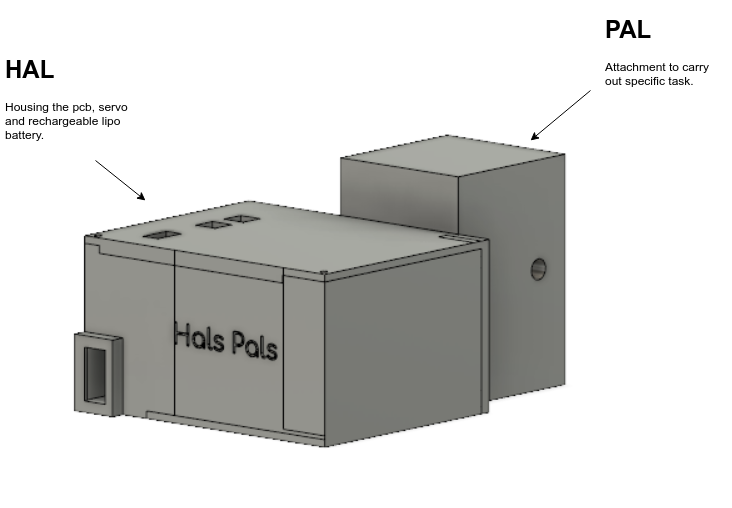
\includegraphics[width=1\textwidth]{images/HALandPAL.png}
               \caption{The components of the robotic adapters.}\label{fig:HalAndPal}
            \end{subfigure}\hfill
            \begin{subfigure}{.5\textwidth}
                \centering
                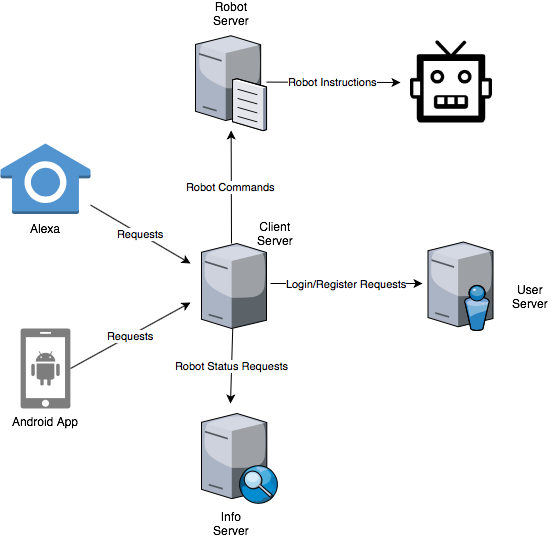
\includegraphics[width=1\textwidth]{images/ArchitectureFlow.png}
              \caption{Flow of information in the system architecture.}\label{fig:ArchitectureFlow}
            \end{subfigure}\hfill
            \end{figure}
        
     {The flow of information in the final system architecture is shown in Figure \ref{fig:ArchitectureFlow}; in the following sections, we shall describe each component in further detail.}


\subsection{Android App}

    \subsubsection{Technical Overview}
    {To allow for the development of new applications targeting the Android mobile operating system, Google released a public Software Development Kit called the Android SDK. This SDK includes all the necessary tools such as debuggers, compilers, etc. \cite{androidsdk}, and allows for development in either Java or Kotlin. The Smart Home Adapters app was developed in Kotlin for the following reasons (all sourced from \cite{kotlin}):}
              \begin{itemize}
                \item Kotlin’s Data Classes reduce the boilerplate code needed to model objects whose primary purpose is to hold data;
                \item Its type system explicitly models nullity, which helps reduce the chance of running into exceptions during integration as the compiler enforces nullity checks where needed;
                \item It is completely interoperable with Java, so it does not adversely impact the number of libraries which can be integrated into the product;
                \item Finally, Kotlin’s lambdas encourage readable and maintainable code by making it easy to associate functions with objects and reducing overhead.
            \end{itemize}
                
    \subsubsection{Architecture}
    {Android applications are typically segmented into different Activities, which correspond to different stages of the application’s lifecycle \cite{androidactivities}. Our application is made up of three such activities developed by HalsPals. The application also uses two activities provided by libraries to handle specific behaviour in the app:}
        \begin{itemize}
                \item RedirectUriReceiverActivity, provided by AppAuth-Android \cite{appauth}. This activity handles the OAuth2.0 authorization process, in which users are taken to a website where they can securely log in, and the resulting session tokens are then fed back to the app.
                \item CaptureActivity, provided by ZXing Android Embedded \cite{zxing}. This activity is launched when the user indicates that they want to scan the robot’s QR code, sets up the camera and parses the QR code, and feeds the result back to the RegisterRobotActivity.
            \end{itemize}
    {Figure \ref{fig:AppFlow} shows the flow between the activities, along with their responsibilities.}
    \begin{figure}[h]
            \begin{center}
               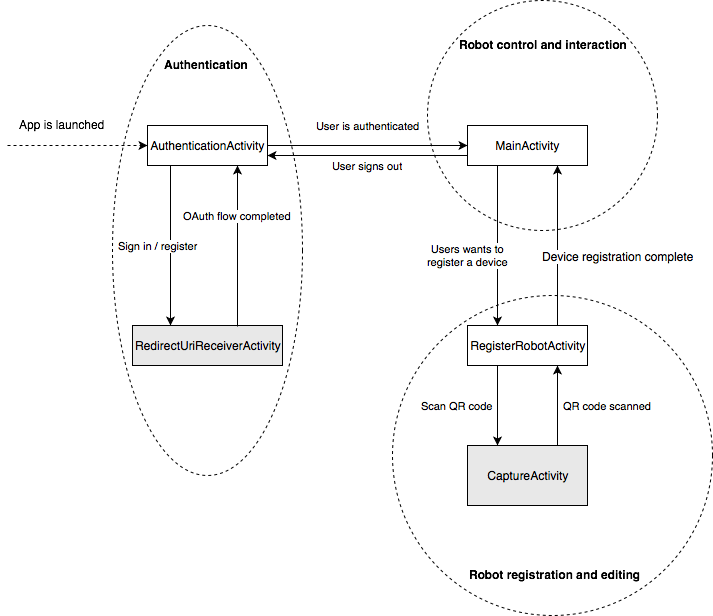
\includegraphics[width=0.5\textwidth]{images/UpdatedAndroidFlow.png}
               \caption{An overview of the app's architecture; the activities provided by libraries are in grey.}
               \label{fig:AppFlow}
            \end{center}
    \end{figure}
        
    \subsubsection{Sending API Requests}
         {In order to communicate with the web server, the app needs to make HTTPS connections. Furthermore, it needs to serialize and deserialize between objects and their JSON representations, for example when fetching the robots associated with the user’s account. Initially a manual approach was taken for this, where AsyncTasks were set up to make the HTTPS connections and the response body was then cast into a JSON object. However, this proved unsatisfactory for a couple of reasons:}
            \begin{itemize}
                \item It becomes difficult to keep track of what the request was for, which is needed in order to handle its results appropriately;
                \item Serializing and deserializing objects is error-prone and involves writing a lot of boilerplate code.
            \end{itemize}
        {Instead, the Retrofit library \cite{retrofit} is used in the final version of the app. With this library, the methods allowed by the REST API are simply defined as an interface; the library then follows the Builder design pattern \cite{builderdesignpattern} to remove the need for boilerplate code. Finally, Retrofit integrates with Gson \cite{gson} to automate the serialization and deserialization process.}

\subsection{Web Services}

\subsubsection{Technical and architectural overview}
       {The web services are comprised of 6 microservices. A microservice architecture was chosen because it:}
            \begin{itemize}
                \item Simplifies security: all components in the system have strict isolated boundaries
                \item Is easy to scale: if one service is experiencing heavy load more instances can be spun up
                \item Simplifies testing: each service is small and has a well-defined interface
                \item Isolates faults: if one service goes down, the others remain unaffected
            \end{itemize}
         The individual microservices are described below:
            \begin{itemize}
                \item \textbf{Client service:} {The client service exposes a public REST API that both Alexa and the Android app use to interact with and control the system.}
                \item \textbf{Info service:} {The info service keeps track of robot ownership and robot details.}
                \item \textbf{Robot service:} {The robot service exposes a websocket server to the robot and provides an interface for the robot to be sent commands.}
                \item \textbf{User server:} {The user server keeps track of registered users’ information.}
                \item \textbf{Account app:} {The account app server provides an authentication mechanism, registering/logging in users and interfacing with our OAuth provider.}
            \end{itemize}
            
        {Golang \cite{go} (also known as Go) was chosen as the development language for the web services, primarily due to the team's previous experience with the language. Furthermore, Go has several benefits:}
            \begin{itemize}
                \item Open-source: Maintained by a wide community \cite{go}
                \item Modern, clean syntax: Reducing code bloat
                \item High level: Quick to develop in
                \item Fast: Go is generally faster than some alternatives such as Python \cite{gofast}
                \item Great concurrency \cite{gocurrency}: important since we are handling multiple clients and robots
            \end{itemize}

\subsubsection{Authentication}
        {For user and Alexa authentication, JSON web tokens were initially used along with a simple login endpoint to exchange credentials for a token. After demo 2, the authentication mechanism was rewritten to support OAuth2.0, a modern standard for secure authentication \cite{oauth}. This was done to support Alexa integration. There are two options for using OAuth:}
            \begin{itemize}
                \item Using a third-party service (Amazon, Google, etc)
                \item Creating your own authentication-providing service
            \end{itemize}
        {The first option is simple as only an API key is required. However, not allowing users to log in with a username and password tied to their HalsPals account might give an unprofessional impression. Instead, the decision was made to implement a custom authentication-providing service.}
       
        {The open source ORY Hydra OAuth server was used to build the authentication-providing service. ORY Hydra does not dictate how you should check credentials or store users, but merely interfaces with OAuth clients. The complexity of OAuth2.0 thus made this task very challenging, despite ORY Hydra's built-in functionality.}
  
\subsubsection{Intra-server communication}
        {Using microservices requires serializing and deserializing every time a message is passed between services. JSON serialisation was used initially, but after some performance analysis it became clear that more time was spent serializing and deserializing than anything else. As a result, the final web service uses gRPC for intra-server communication. gRPC combines RPC (remote procedure calls) with protocol buffers - fast binary serialisation, and allowed for response times averaging around 70ms.}

\subsubsection{Deployment}
        {One downside of microservices is how difficult they are to deploy. Cloud hosted Docker \cite{docker} containers automated with continuous integration and deployment were used to alleviate this problem. Whenever a new feature or bug fix would be merged into the \textit{webserver} branch of our repository, CircleCI \cite{circleci} would run unit tests and linters. If these checks passed, CircleCI would then build Docker images for each microservice and push it to Dockerhub. Finally, an instance of Watchtower \cite{watchtower} running on the web server would detect new versions of images pushed to Dockerhub, download the updated images and restart the microservices.}

\subsection{Alexa Integration}
   \subsubsection{Architectural overview}
   Amazon's Alexa provides a set of built-in capabilities, referred to as \textit{skills}. Each skill provides a predefined voice interaction model to the Alexa cloud; using this model, the Alexa cloud interprets the customer's utterances and then sends processed messages back to the skill to handle. Finally, the skill sends a response back to the Alexa cloud to indicate sucess or failure. 
  
  \begin{figure}[h]
            \begin{center}
               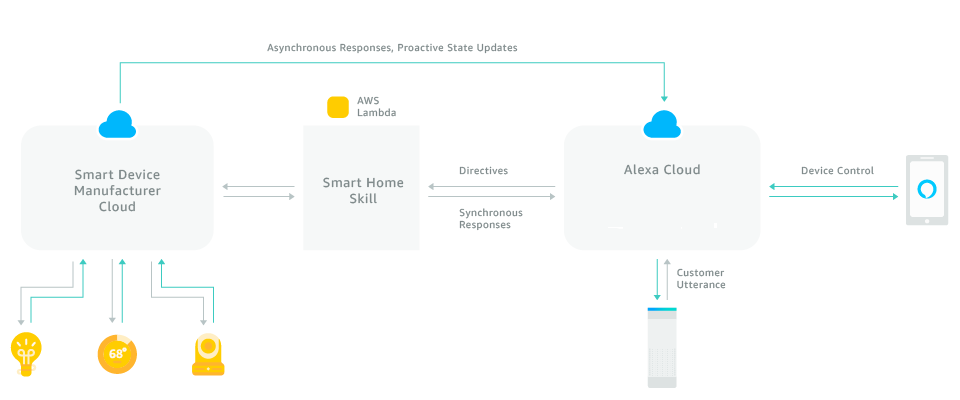
\includegraphics[width=0.5\textwidth]{images/Alexa.png}
               \caption{Alexa basic workflow}
               \label{fig:alexa work flow}
        \end{center}
    \end{figure}
    
    There are several kinds of skill models provided by Alexa; the HalsPals extension uses the Smart Home skill API. This API comes with a predefined voice interaction model, making supporting voice control easy regardless of the use case. The cloud uses this voice interaction model to process the user's commands before sending them to the HalsPals extension, which then parses these and sends requests onward to the HalsPals REST API as appropriate. However, it should be noted that the Smart Home skill API does not allow for custom responses sent back to the Alexa cloud. As such, the vocal responses from Alexa are simplistic.
    
    
    \subsubsection{Authentication}
    
    The first step in implementing the smart home skill is to set up the authentication mechanism. Using OAuth, the server will provide an \textit{Authorization URI}, a \textit{Client ID}, a \textit{Client Secret}, an \textit{Access Token URI} and a \textit{scope} to Alexa. These details are then used to set up the Alexa console account link, which is the bridge that connects the lambda function to our client server.
    
    When the user launches their Alexa app, they can install the HalsPals skill. After enabling this skill, an account link process is opened; this will direct the user to the HalsPals OAuth login page. After having validated the user's credentials, the Alexa cloud will automatically send an AcceptGrant directive to the skill. This directive contains the access token for Alexa and the skill code this token uses to communicate with the server. Thus, authentication of the user is complete.
    
    \begin{figure}[h]
     \begin{subfigure}{.5\textwidth}
            \centering
                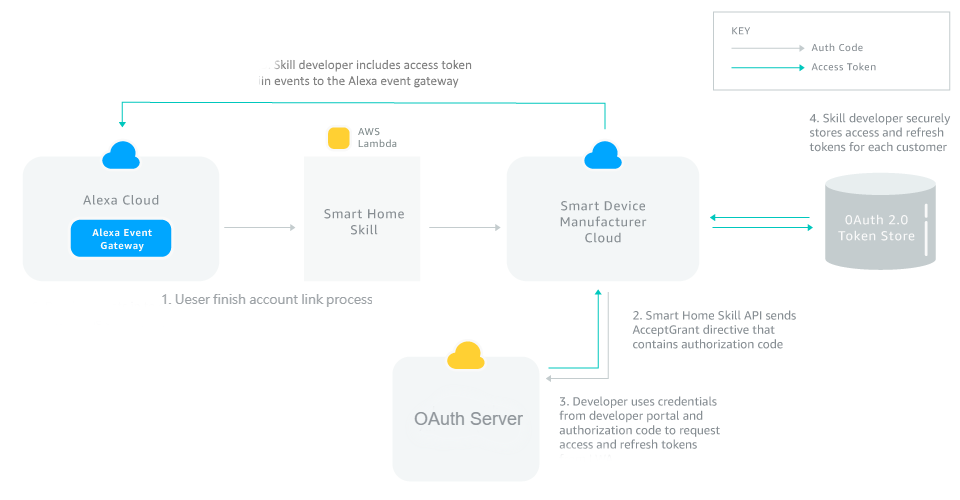
\includegraphics[width=1\textwidth]{images/auth.png}
                \caption{Alexa authentication workflow}
               \label{fig:alexa autthentication flow}
            \end{subfigure}\hfill
            \begin{subfigure}{.5\textwidth}
                \centering
                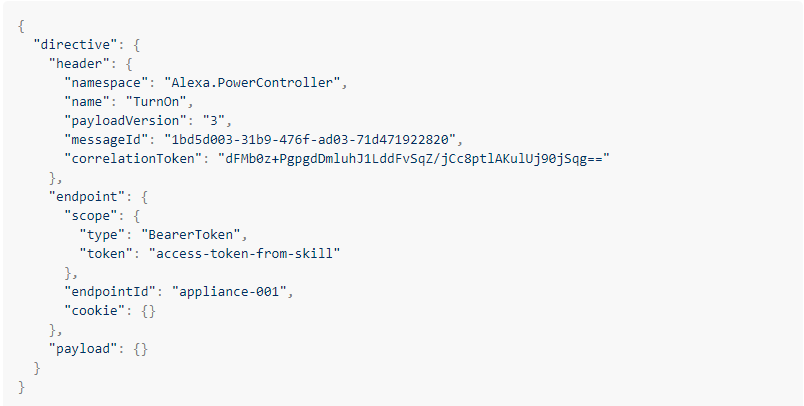
\includegraphics[width=1\textwidth]{images/Alexarequest.png}
                \caption{Example processed message after uttering "Alexa, turn on the switch". Here the switch has been set up with unique ID appliance-001.}
               \label{fig:alexa switch flow}
            \end{subfigure}\hfill
        \caption{Alexa examples}
    \end{figure}
    
    \subsubsection{Implementing the skill} Other than setting up the authentication, the actual implementation of the skill mainly comes down to setting up the request handler. This handler has two main responsibilities: handling the incoming requests from the Alexa Cloud, and sending responses indicating success or failure back once it has done so. The format of the requests is always a JSON; the fields which we are interested in are:
    \begin{itemize}
        \item The namespace of the API being used
        \item The name of the action taken
        \item The endpoint identifier, i.e. which device the user wants to interact with
        \item The scope's token, which is the access token to use for the request.
    \end{itemize}
    What varies between the requests is the information contained in these components; this is what the skill needs to handle. For example, Figure \ref{fig:alexa switch flow} shows an "Alexa, turn on the switch" request. In this case, the handler needs to parse the JSON in order to figure out that a robot control request is desired, how the control the robot, which robot to control, and who the user is. It is then up to the handler to construct an accurate HTTPS request to the HalsPals REST API to carry out this task. Once it has done so, it waits to hear back from the HalsPals server before sending a JSON file back to the Alexa cloud to indicate whether the request was carried out successfully, following a strict format set by Alexa.
    
\subsection{3D-Printing and 3D-Milling}
    To minimize the form factor and weight of the adapters, the final product uses largely 3D-printed designs. In this section, we will look at the designs of each component in detail.
    
    % we don't have room for vertical space sadly :( indents will have to do \hfill\\
    
    \subsubsection{Light switch PAL}
        Initially, LEGO parts were used to construct the light switch PAL. A lamp was employed to test this construction; the mechanism worked well. However, this construction was bulky in appearance, and proved too heavy to attach to a wall easily. After some trial and error, a more adaptable, smaller design was conceived, where the servo was mounted in a suitable position using a gear and its gear racks. This allowed the mechanism to be precise, lightweight, and far more durable. Finally, once the HAL design had been finished, this design was updated slightly to connect to the HAL seamlessly.
        Figure \ref{fig:switchPALs} shows all three of these iterations.
         
          \begin{figure}
            \begin{subfigure}{.3\textwidth}
                \centering
                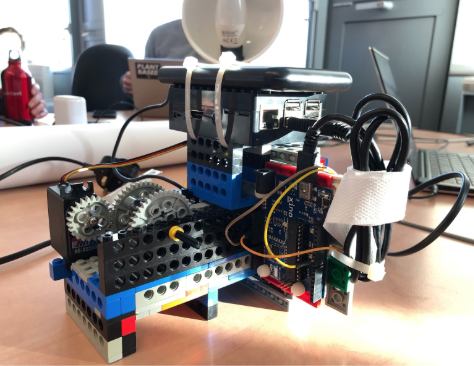
\includegraphics[width=0.7\textwidth]{images/Light1.png}
                \caption{First iteration}
            \end{subfigure}\hfill
            \begin{subfigure}{.3\textwidth}
                \centering
                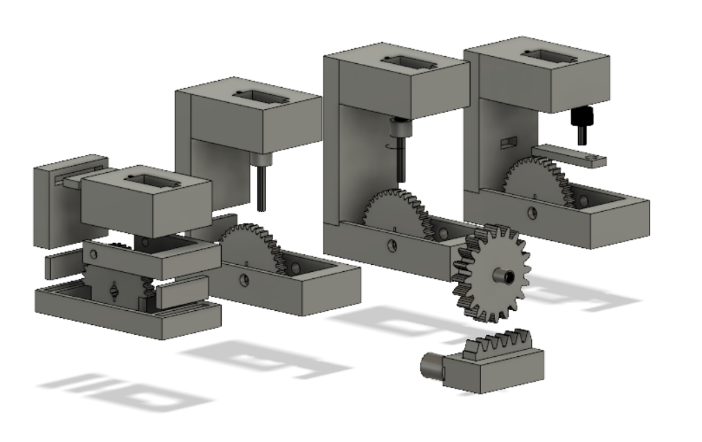
\includegraphics[width=0.7\textwidth]{images/Light2.png}
                \caption{Second iteration}
            \end{subfigure}\hfill
            \begin{subfigure}{.3\textwidth}
                \centering
                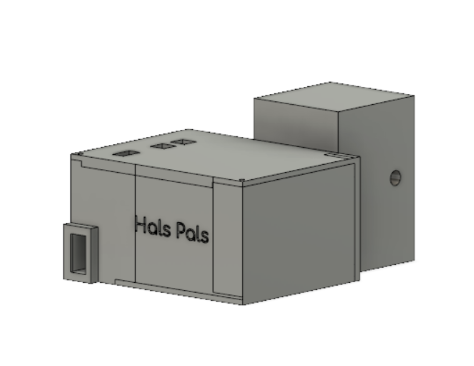
\includegraphics[width=0.6\textwidth]{images/Light3.png}
                \caption{Third iteration}
            \end{subfigure}
        \caption{Light switch PAL iterations}
        \label{fig:switchPALs}
        \end{figure}
         
   % \hfill\\
   
    \subsubsection{Thermostat PAL}
        Once again, LEGO was initially used to construct this PAL. The adapter would change the temperature by moving the servo to the desired angle; a suction cup attached to the server would twist the thermostat's knob. However, this construction required a large frame to keep the suction cup in place, which made it unsuitable for our use case. The thermostat PAL was then redesigned using 3D milled acrylic parts, which are light and strong, along with M4 and M6 bolts, nuts, washes and some 3D printed parts. With this construction, the size of the frame is adjustable to fit different thermostats, and the position of the knob grip can be adjusted along all three dimensions. This design proved suitable for the mechanical thermostats it was tested on, and only saw minor changes in the form of a new HAL-to-PAL connector once the HAL design was finished. Finally, the accuracy of the PAL was increased by adding reusable sticky gel to the inside of the suction cup, improving its grip on the thermostat knob. Figure \ref{fig:thermoPALs} shows all three of these iterations.
            
        \begin{figure}
            \begin{subfigure}{.3\textwidth}
                \centering
                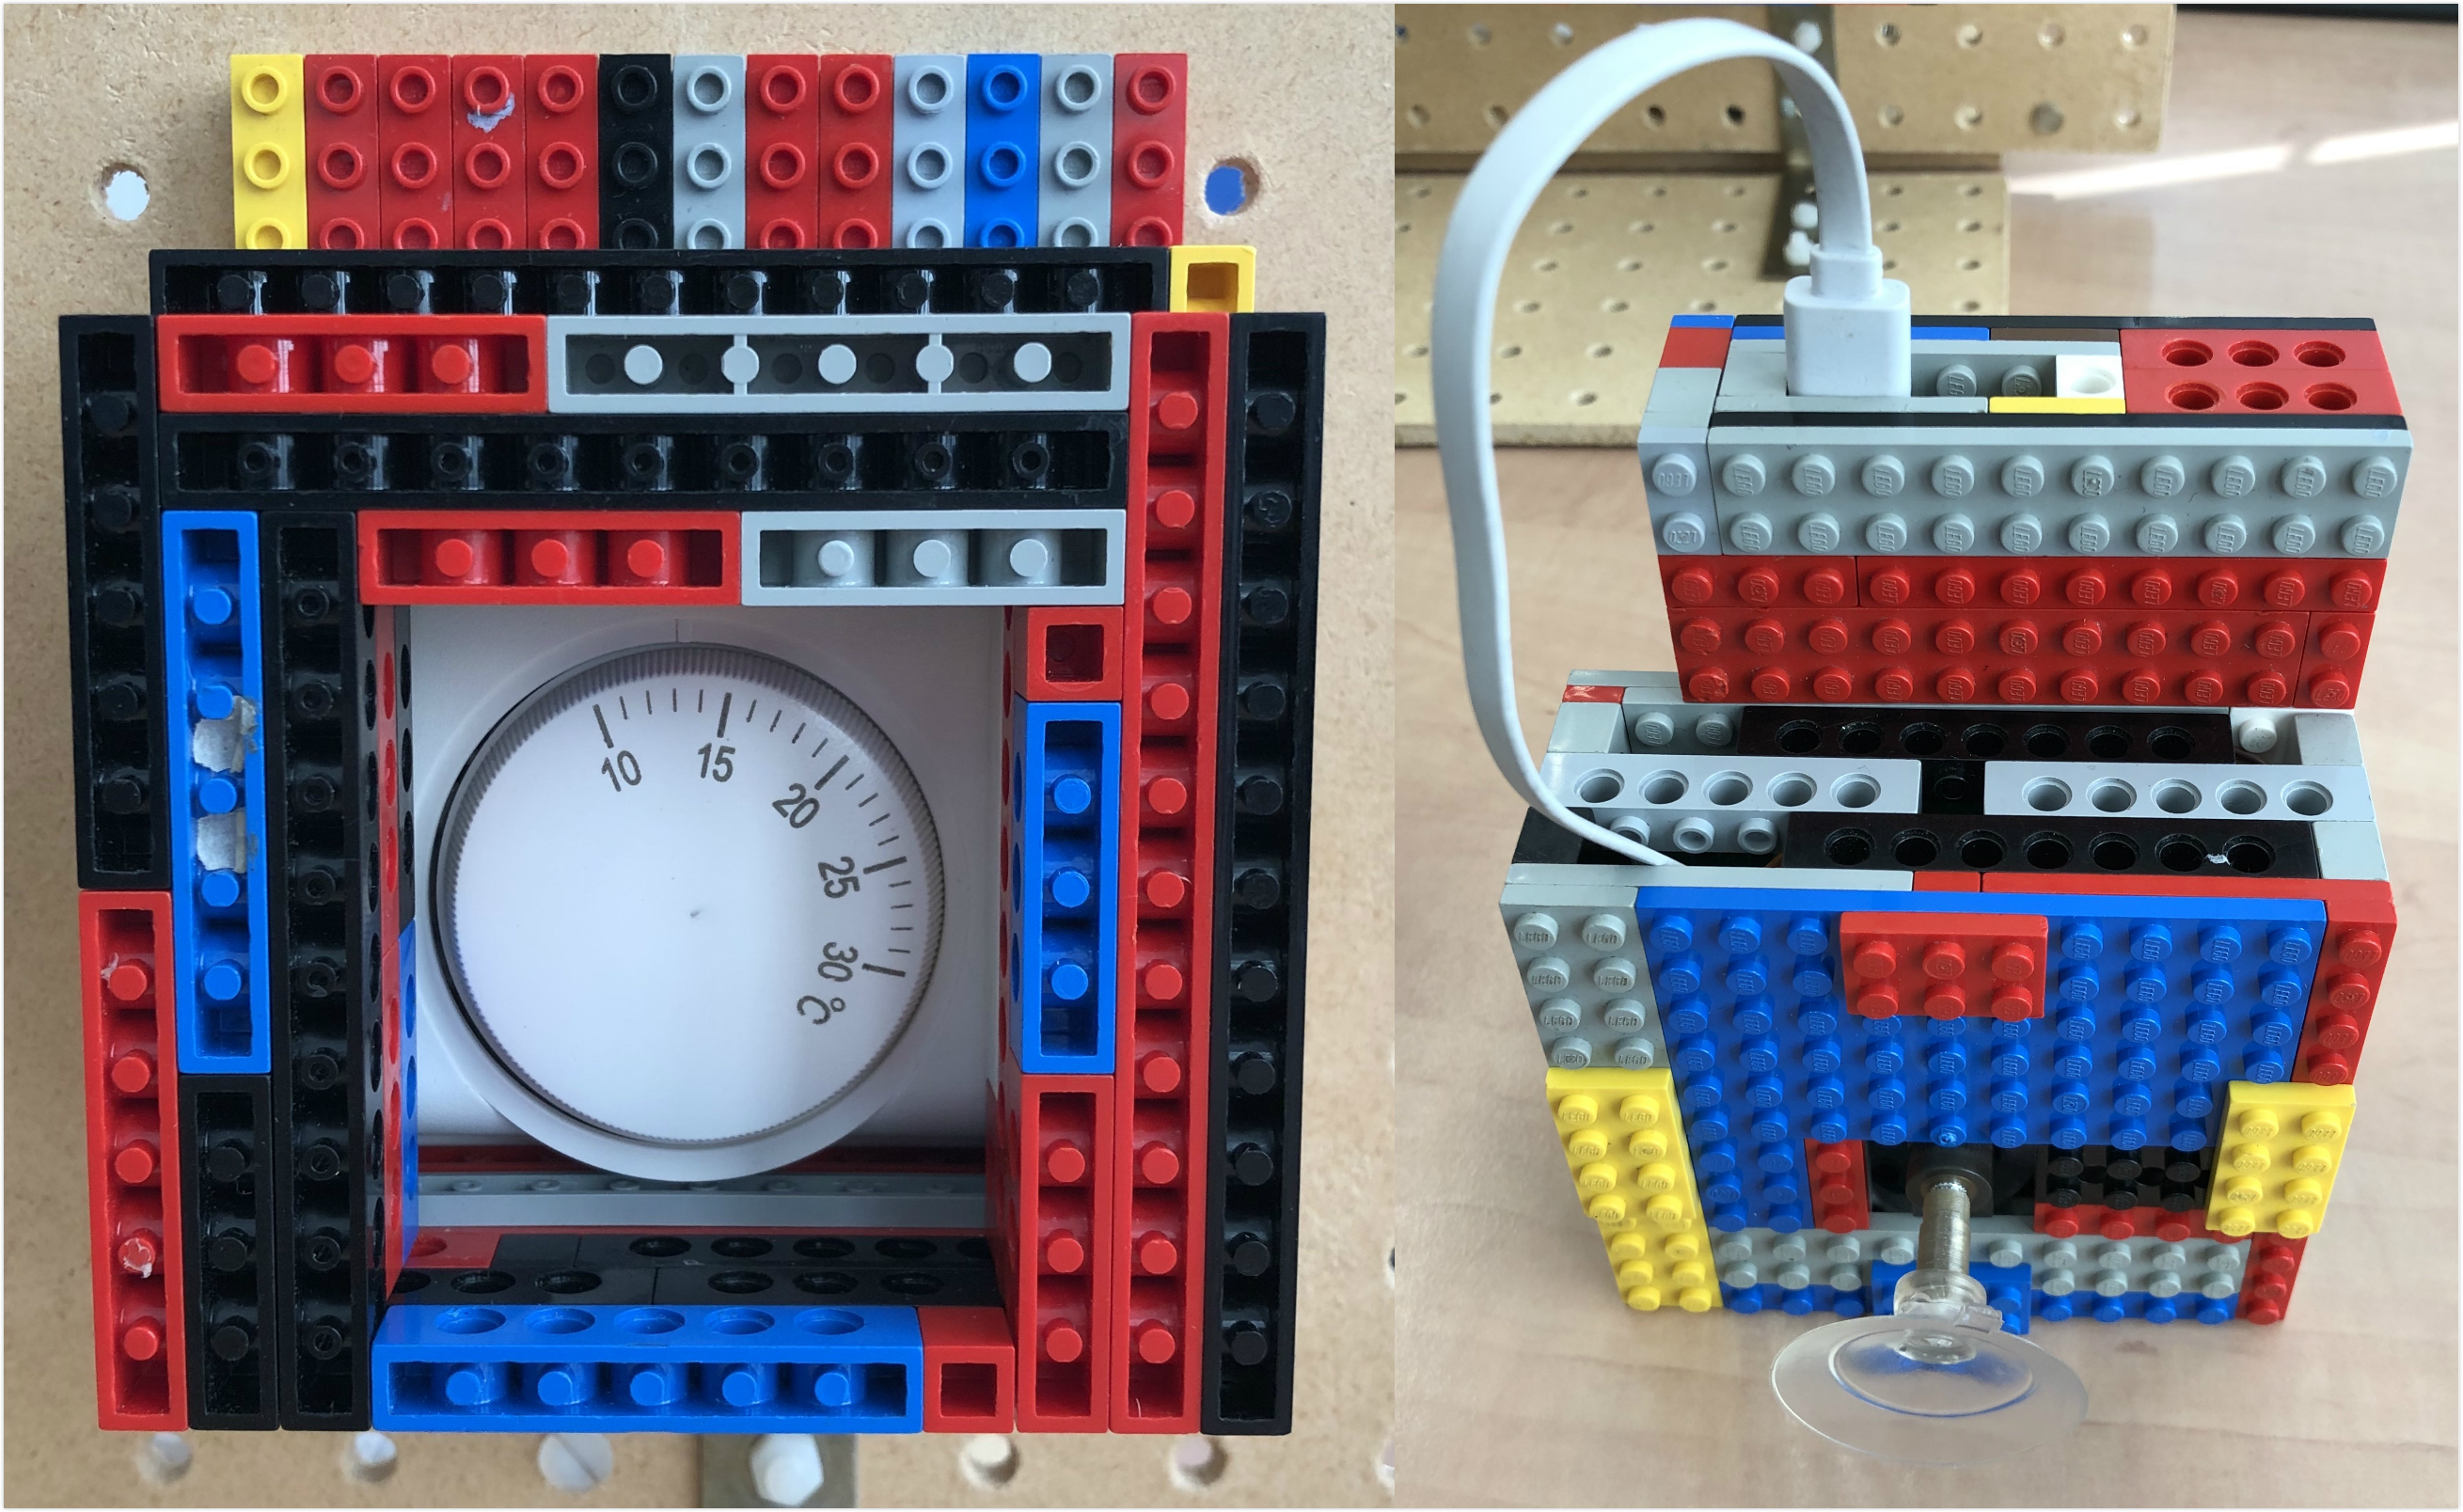
\includegraphics[width=1\textwidth]{images/Thermo1.jpg}
                \caption{1st iteration}
            \end{subfigure}\hfill
            \begin{subfigure}{.3\textwidth}
                \centering
                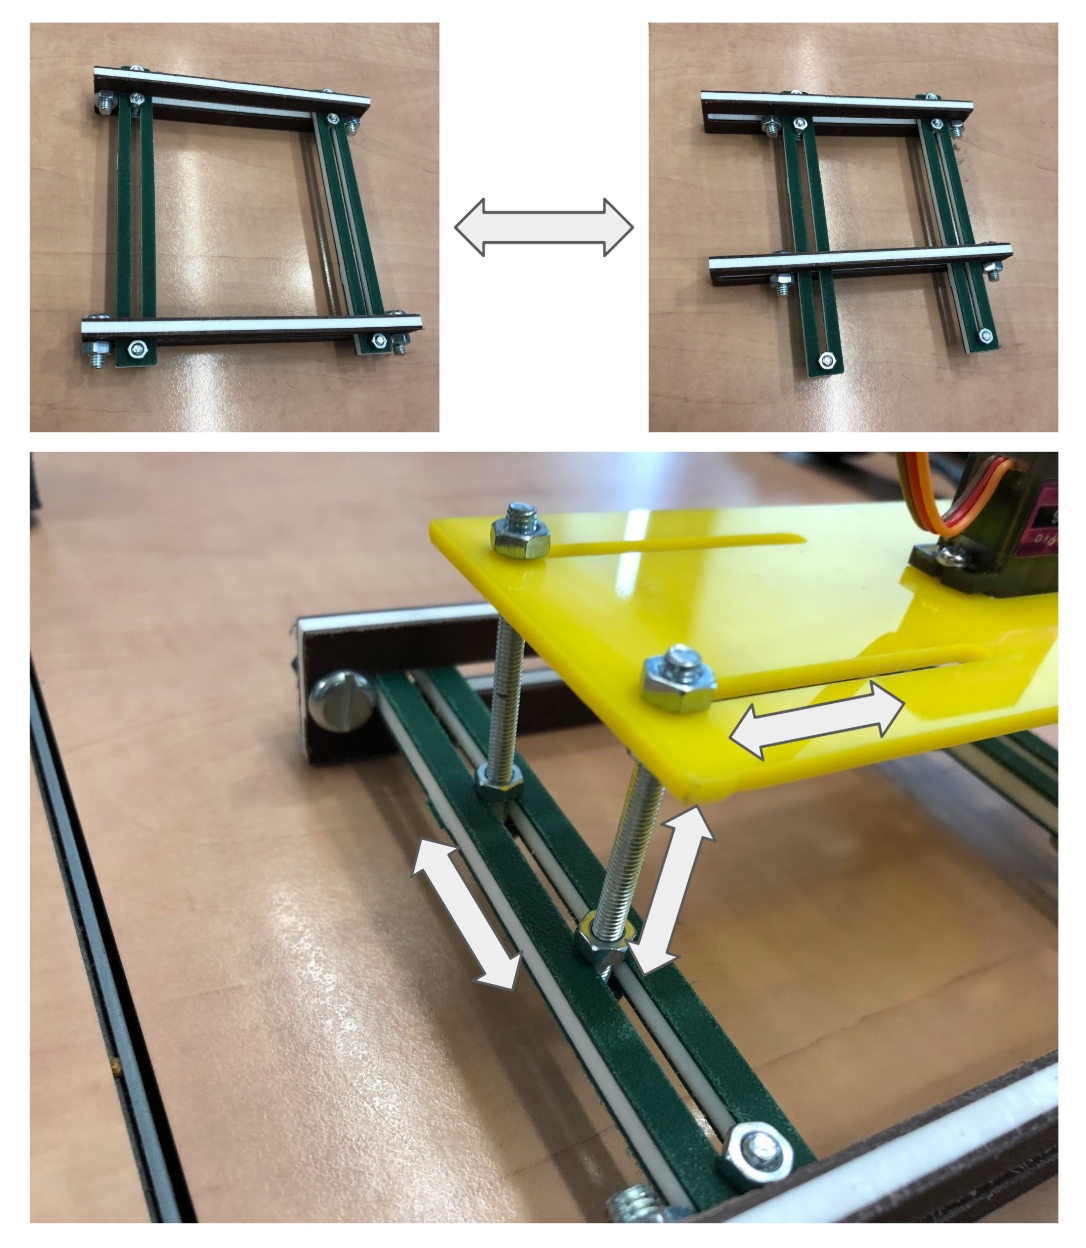
\includegraphics[width=0.7\textwidth]{images/Thermo2.png}
                \caption{2nd iteration}
            \end{subfigure}\hfill
            \begin{subfigure}{.3\textwidth}
                \centering
                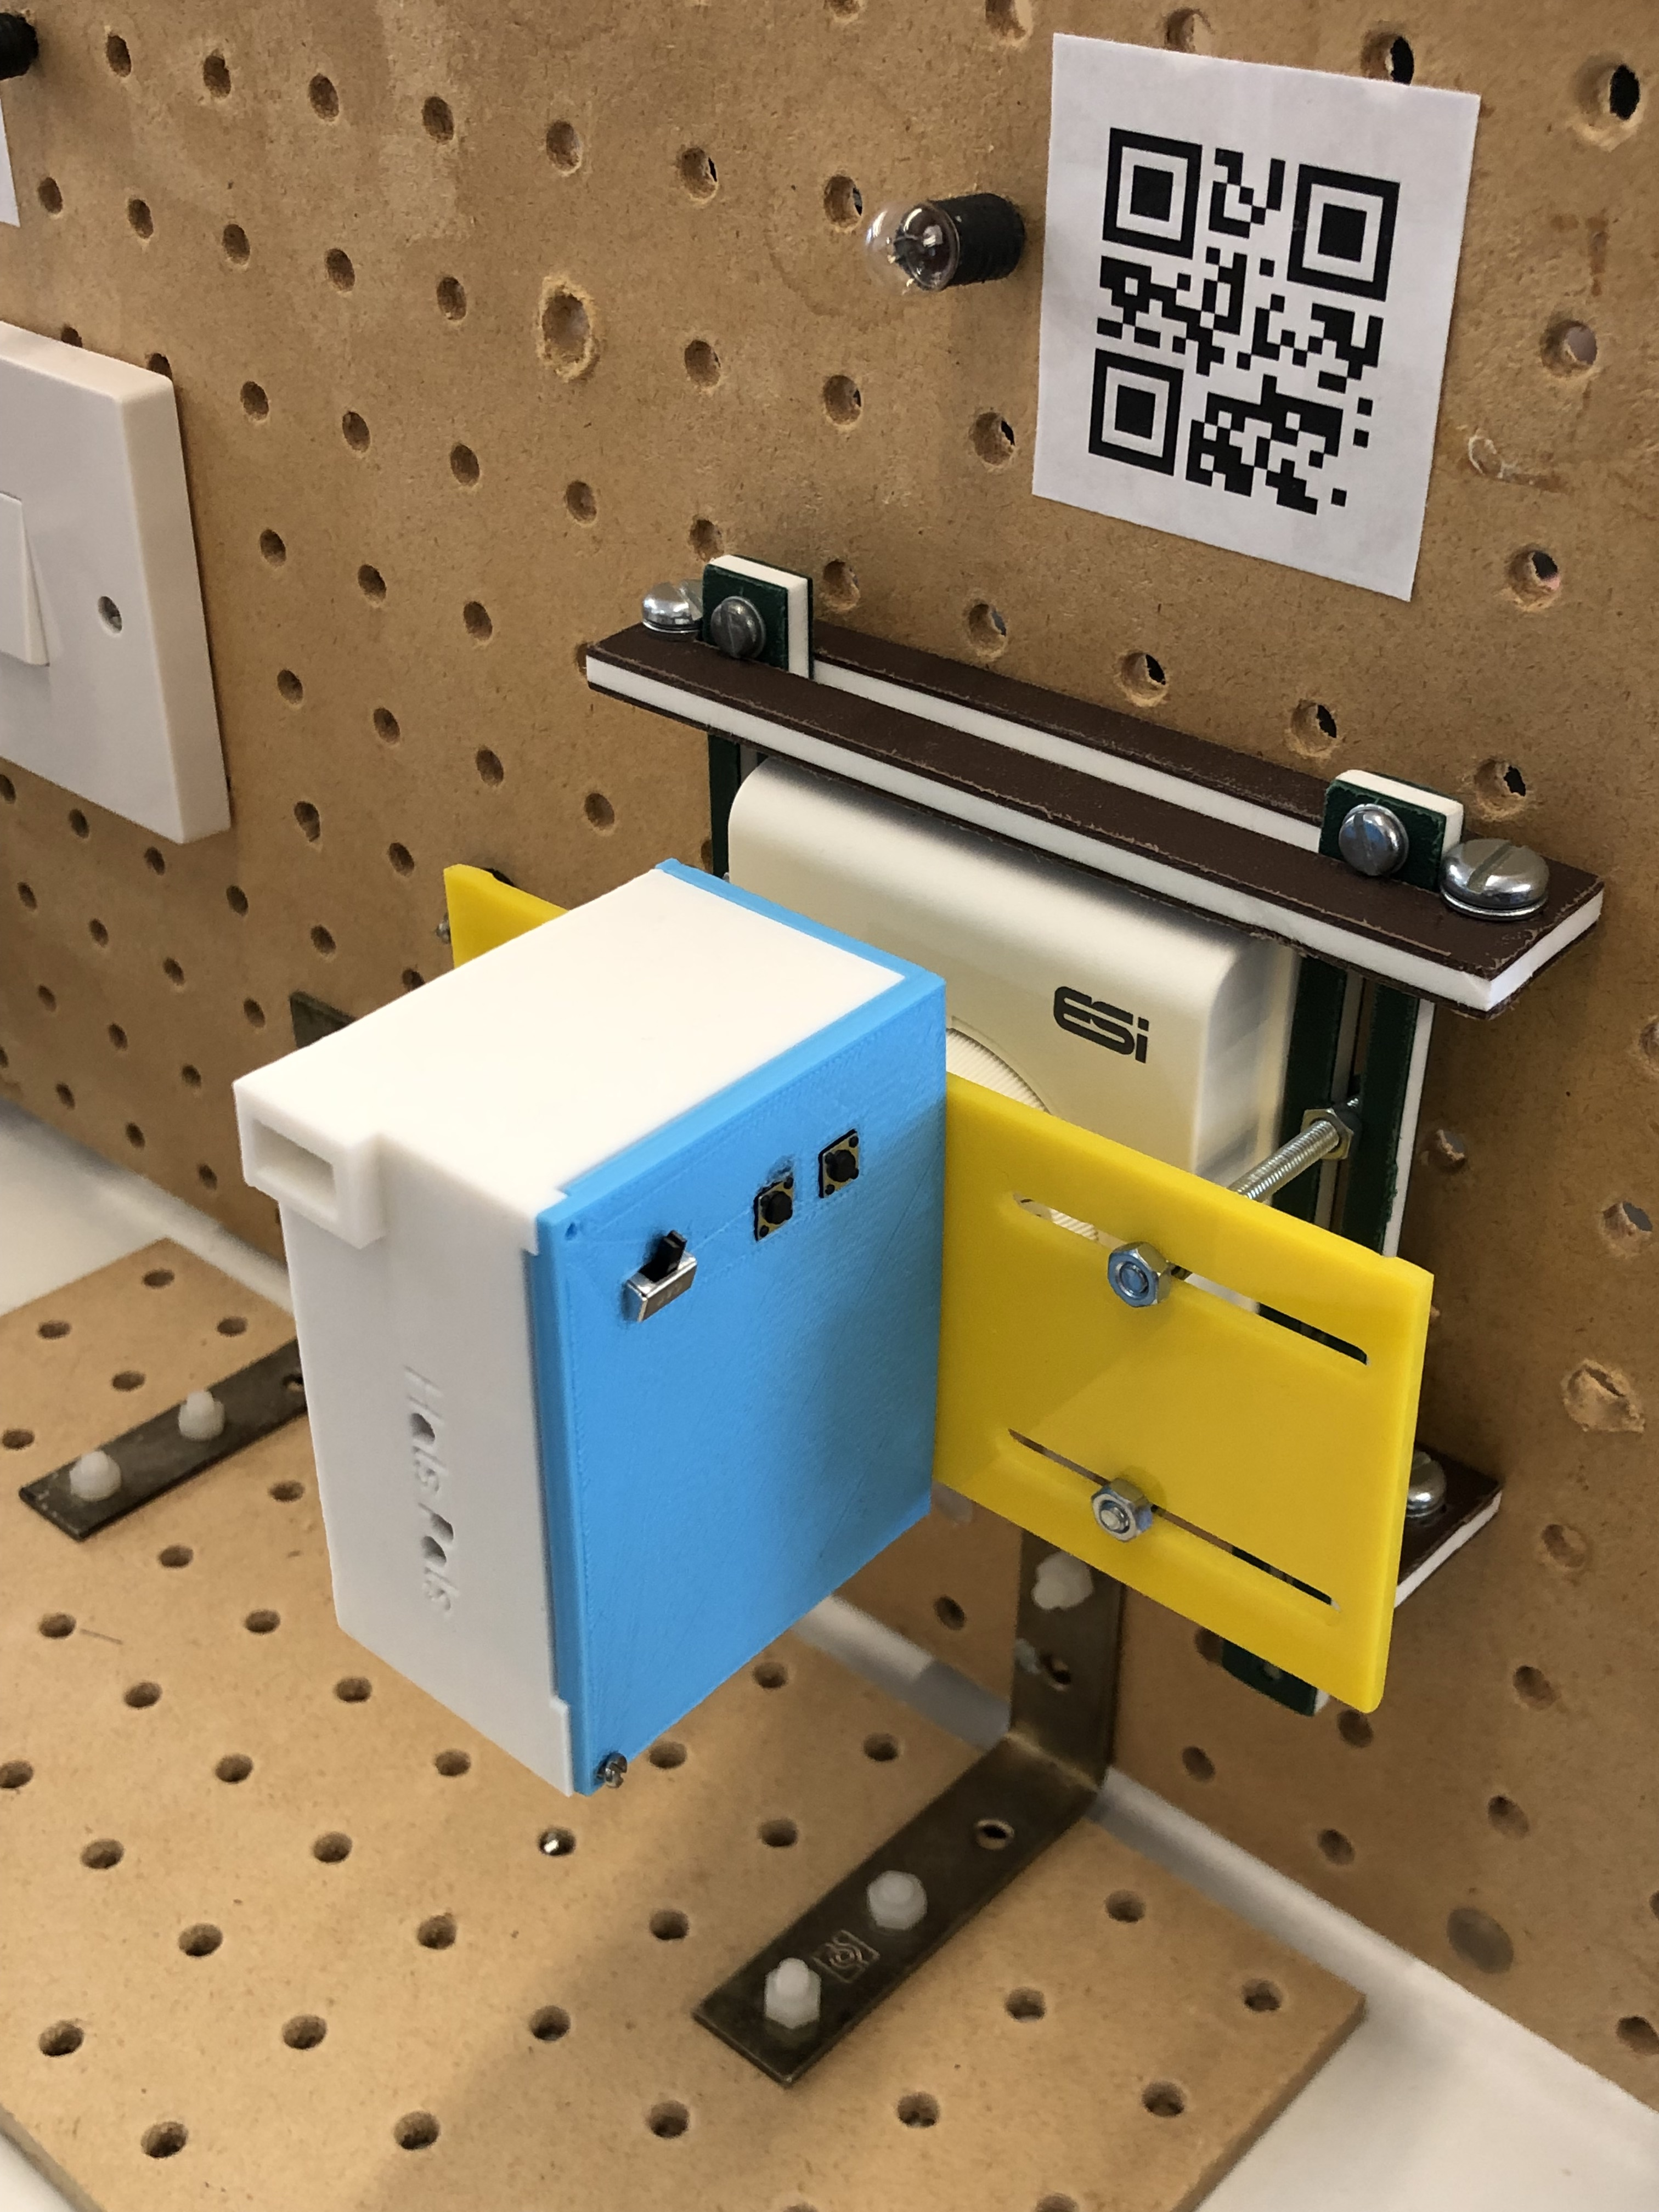
\includegraphics[width=0.6\textwidth]{images/Thermo3.jpg}
                \caption{3rd iteration}
            \end{subfigure}
        \caption{Thermostat PAL iterations}
        \label{fig:thermoPALs}
        \end{figure}

        
   % \hfill\\
    \subsubsection{Bolt Lock PAL}
        We started to make the Bolt Lock PAL before the third demo and we had the experience of designing the other two PALS, so we decided to start it with 3D print directly. Since the motion mode of the bolt lock is simple linear motion. We put a gear rack and a gear connected to the servo in it. After we had the mechanism working, we updated the Bolt Lock PAL leaving a connector to the HAL instead of having the servo in it directly.
        
        \begin{figure}
            \begin{subfigure}{.3\textwidth}
                \centering
                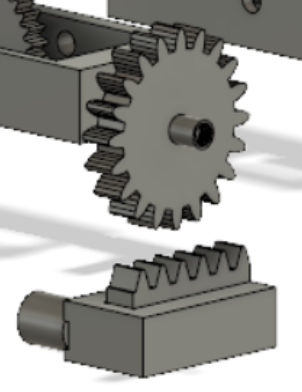
\includegraphics[width=0.5\textwidth]{images/Boltlock1.png}
                \caption{1st iteration of Bolt Lock}
            \end{subfigure}\hfill
            \begin{subfigure}{.3\textwidth}
                \centering
                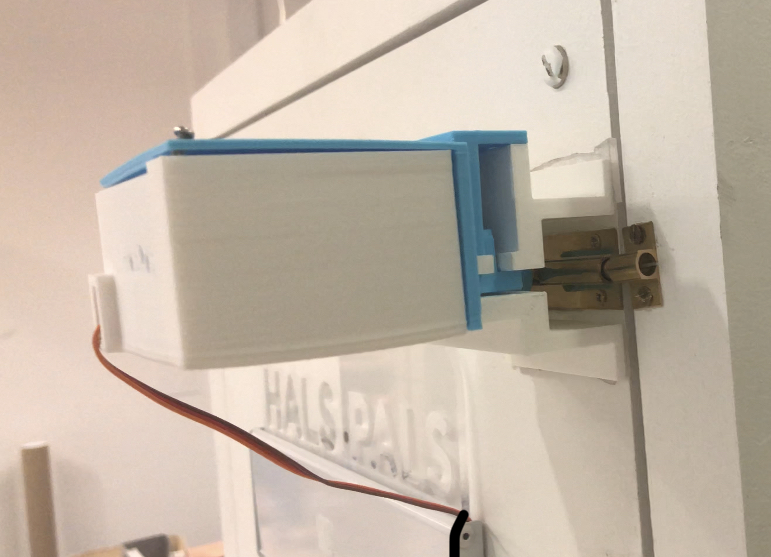
\includegraphics[width=0.6\textwidth]{images/Boltlock2.jpg}
                \caption{2nd iteration of Bolt Lock}
            \end{subfigure}\hfill
        \begin{subfigure}{.3\textwidth}
                \centering
                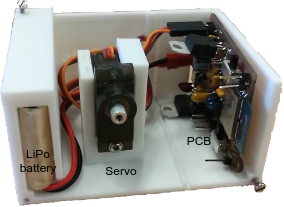
\includegraphics[width=0.6\textwidth]{images/HAL.png}
                \caption{HAL's Layout}
                \label{fig:hal}
            \end{subfigure}\hfill
        \caption{Bolt lock PAL and HAL designs}
        \end{figure}
        
        
   % \hfill\\
    \subsubsection{HAL}
    The primary functionality of the HAL is to hold all the electronic components, and to lock the servo into place; this is shown in Figure \ref{fig:hal}. This design leaves some space between the components in order to protect the battery from overheating due to the board warming up. Finally, the HAL design features spaces for button control and battery charging, as can be seen in Figure \ref{fig:HalAndPal}.

        
    
\subsection{Hardware}
        \subsubsection{General Overview}
        {The hardware consist of a servo motor, a controller board to control the servo, and power source. Simple as that sounds, the hardware went through many iterations throughout the length of the project in order to minimize the form factor and power draw. Here we discuss the final approach taken, also highlighting why previous attempts were abandoned.}
        
        \subsubsection{Servomechanism}
        {The Hitec HS-322HD Standard Heavy Duty Servo was used in early designs of the HAL, as its maximum torque of 3.7 kgf-cm was beyond adequate for the first light switch adapter. However, further testing revealed that only 2kgf-cm was needed to turn the switch on or off. The Tower Pro MG90S Metal Gear Servo was therefore used instead in the final iteration, as it brought a significant size and weight reduction while still providing enough torque to actuate the adapters.}

        \begin{center}
            \begin{tabular}{||c | c | c | c||} 
                 \hline
                 Servo & Weight(g) & Dimensions(mm) &  Maximum Torque (kgf-cm) \\ [0.5ex] 
                 \hline\hline
                 Hitec HS-322HD\cite{servo1}& 42.8 & 39.9x19.8x36.3 & 3.7 \\ 
                 \hline
                 Tower Pro MG90S\cite{servo2} & 13.4 & 22.5x12.0x35.5 & 2.2 \\
                 \hline
            \end{tabular}
        \end{center}
     
        \subsubsection{Electronics}
      
       Initially an Arduino Uno R3 and a Raspberry Pi were the only electronics available. With plans to switch to a NodeMCU ESP8266 development board in the future to reduce the system's size, the Arduino Uno was chosen for early prototypes as the source code could be reused for the NodeMCU, using a plugin to the Arduino IDE \cite{espplugin}. The Raspberry Pi’s function was simply to connect the system to WiFi \cite{pi2wifi}. Figure \ref{fig:electronics1}) shows how the initial system was connected, using the Hitec HS-322HD servo and the ANSMANN Powerbank 5.4 portable battery.
            
         \begin{figure}
            \begin{subfigure}{0.5\textwidth}
                \centering
                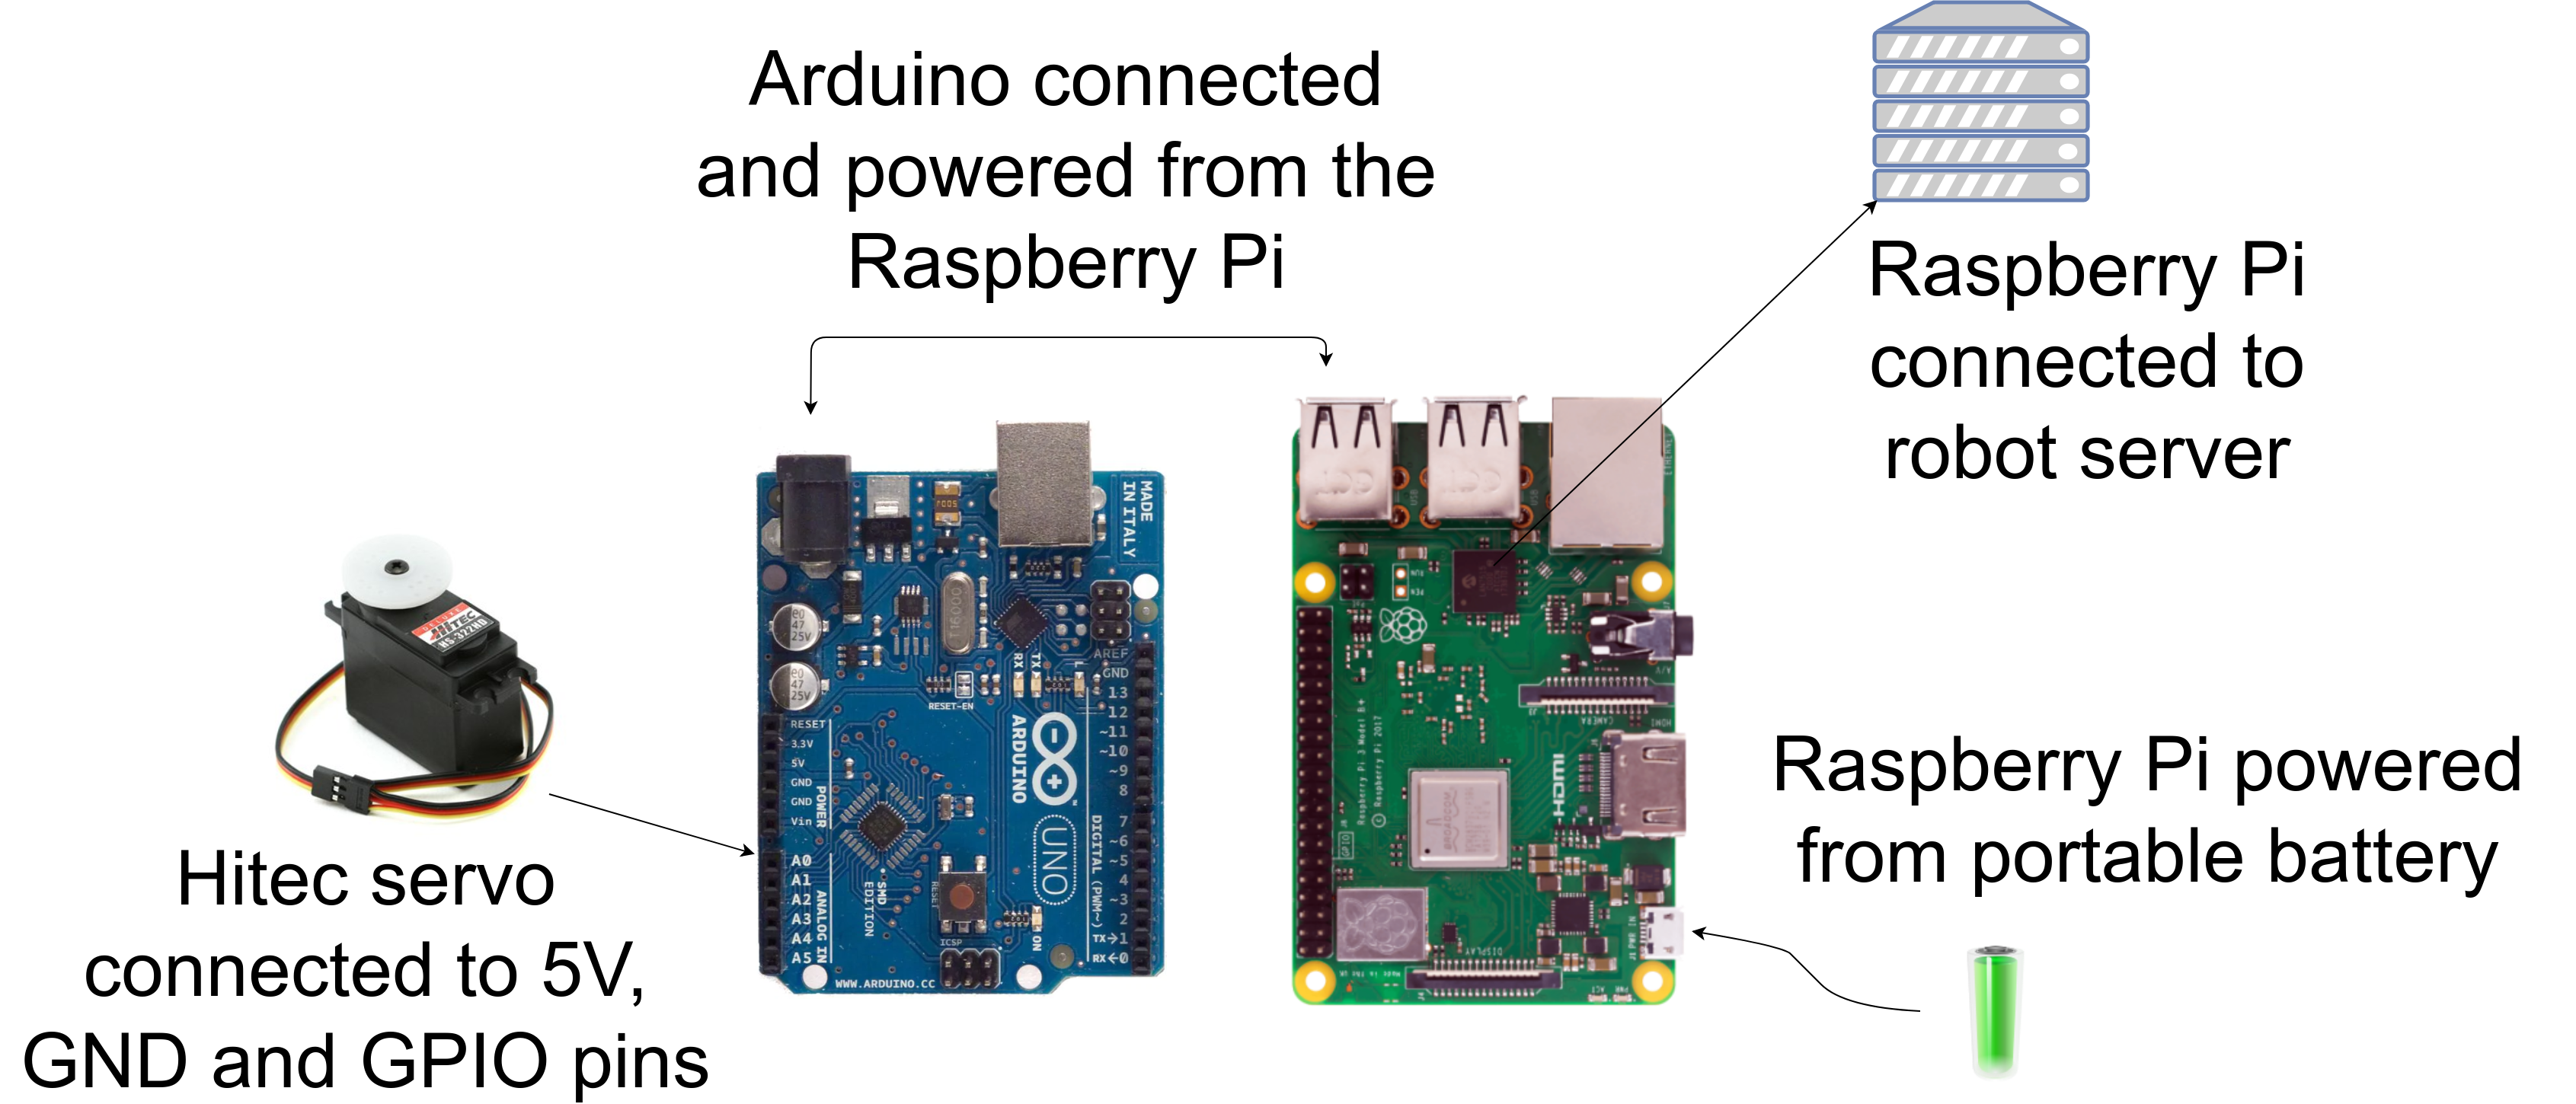
\includegraphics[width=1\textwidth]{images/Piduino.png}
                \caption{First iteration}
                \label{fig:electronics1}
                
            \end{subfigure}\hfill
            \begin{subfigure}{.5\textwidth}
                \centering
                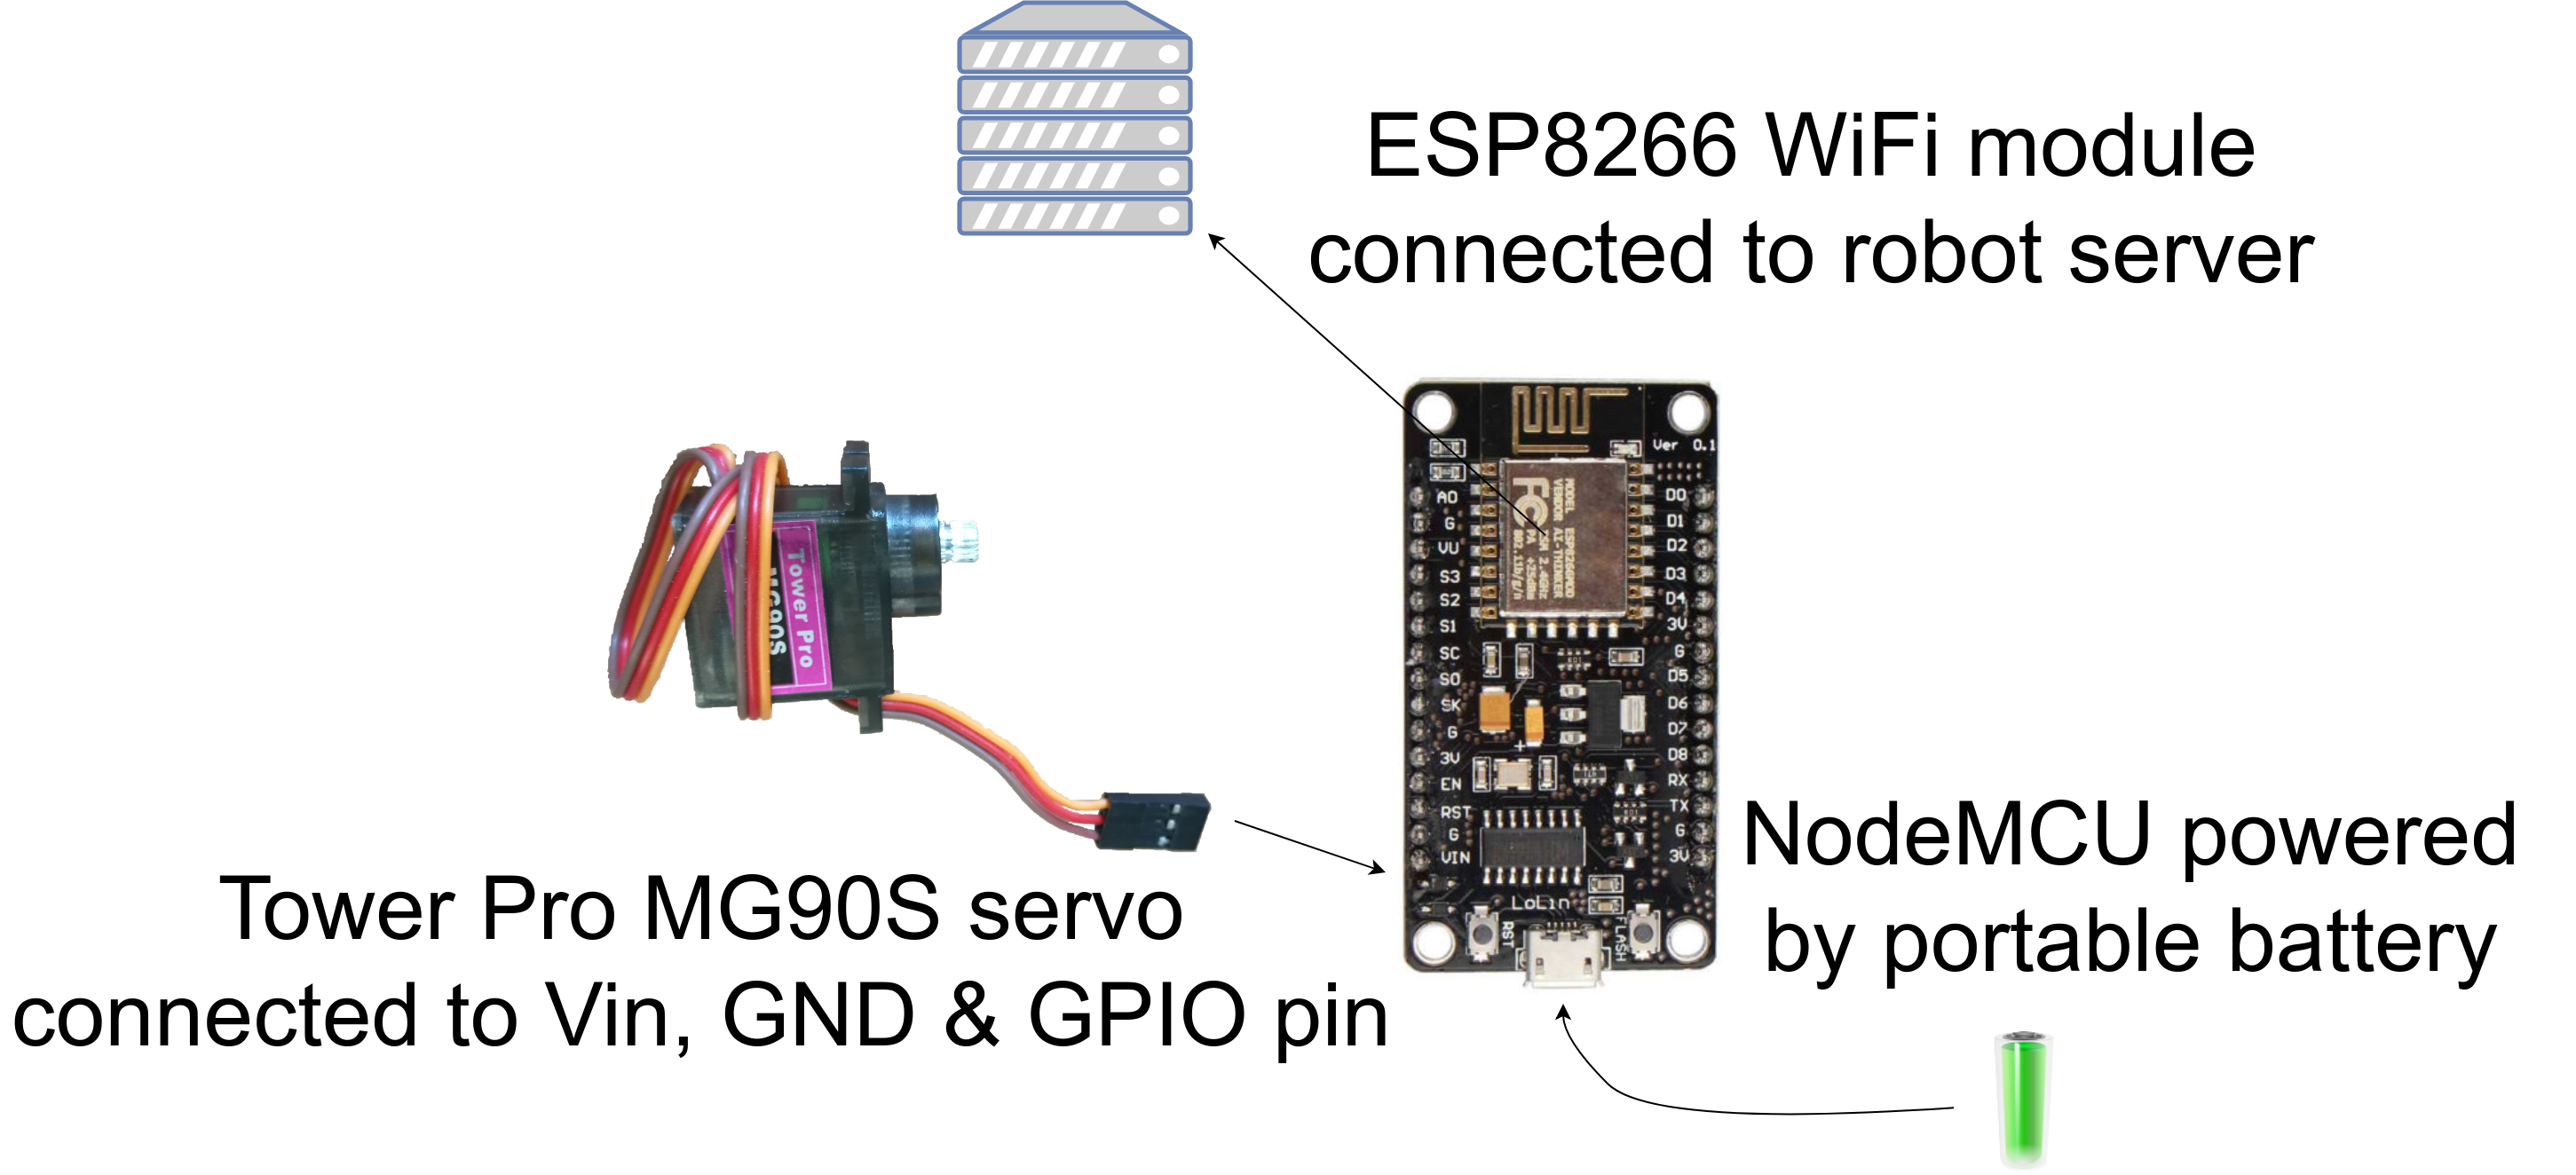
\includegraphics[width=.8\textwidth]{images/NodeMCyou.png}
                \caption{Second iteration}
                \label{fig:electronics2}
            \end{subfigure}\hfill
        \caption{Initial hardware iterations}
        \end{figure}
        
        Once NodeMCUs had been brought in, a second iteration of the hardware was developed (shown in Figure \ref{fig:electronics2}. The code used to control the robots remained the same, but this time the power and WiFi access were both connected directly to the NodeMCU. This proved very challenging, as one of the main difficulties with regards to all ESP8266 WiFi modules is connecting them to a WPA2 Enterprise network (as has been discussed widely within the ESP8266 community \cite{wpa2}). Due to university building regulations disallowing WiFi access points, we needed to brave this challenge and connect the robots to Eduroam. This was finally achieved using the latest version of the official NONOS ESP8266 SDK \cite{nonos}, however it required quite some trickery: the module needed to be flashed with the NONOS SDK at a certain position in memory \cite{sdkstart} (depending on the module's memory size).
        
        A multimeter was used to test the current draw of this design. On idle it ran at approximately 70mA, peaking to 140mA whilst sending and receiving WiFi packets and 400mA whilst moving the servo. With the Ansmann Powerbank’s battery capacity of 5400mAh the system could thus last up to 3 days (when utilising the ESP8266’s deep sleep function \cite{deepsleep} this can be increased significantly to 12.5 days).
        {Having carried out this testing, we realized two things:}
            \begin{itemize}
                \item The NodeMCU, though great for development, was overkill for our application. Switching to a simple ESP8266 WiFi module would reduce power consumption even more, as well as size.
                \item The Ansmann Powerbank portable battery was bulky and heavy; the Conrad Energy 1000mAh Lithium Polymer Battery would make for a smaller, lighter option.
            \end{itemize}
        {Although switching to this solution left us with a few other issues:}
            \begin{itemize}
                \item The Conrad LiPo battery outputs 3.7V. Our Tower Pro MG90S servo needed a minimum of 4.8V to function, and all ESP8266 WiFi modules require a strict 3.3V to not damage the module.
                \item We had no way of recharging the LiPo battery, without adding additional bigger boards to our design.
            \end{itemize}
            
     {A custom PCB was designed to alleviate these issues. This kept the system small and compact, and fully enclosed in our 3D printed HAL. With reference to the units in the schematic our reasons for integrated circuits choices can be found in Figure \ref{fig:pcbsch}.
     
      
         \begin{figure}[h]
            \begin{center}
               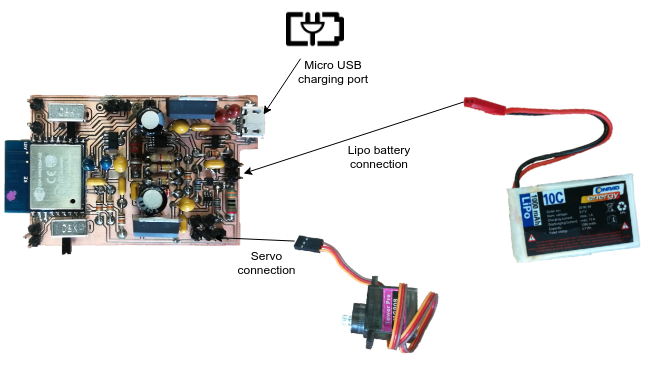
\includegraphics[width=0.6\textwidth]{images/PCB-Connection.png}
               \caption{PCB Connections}
               \label{fig:pcb}
            \end{center}
        \end{figure}
     
     
        
         \begin{figure}[h]
            \begin{center}
               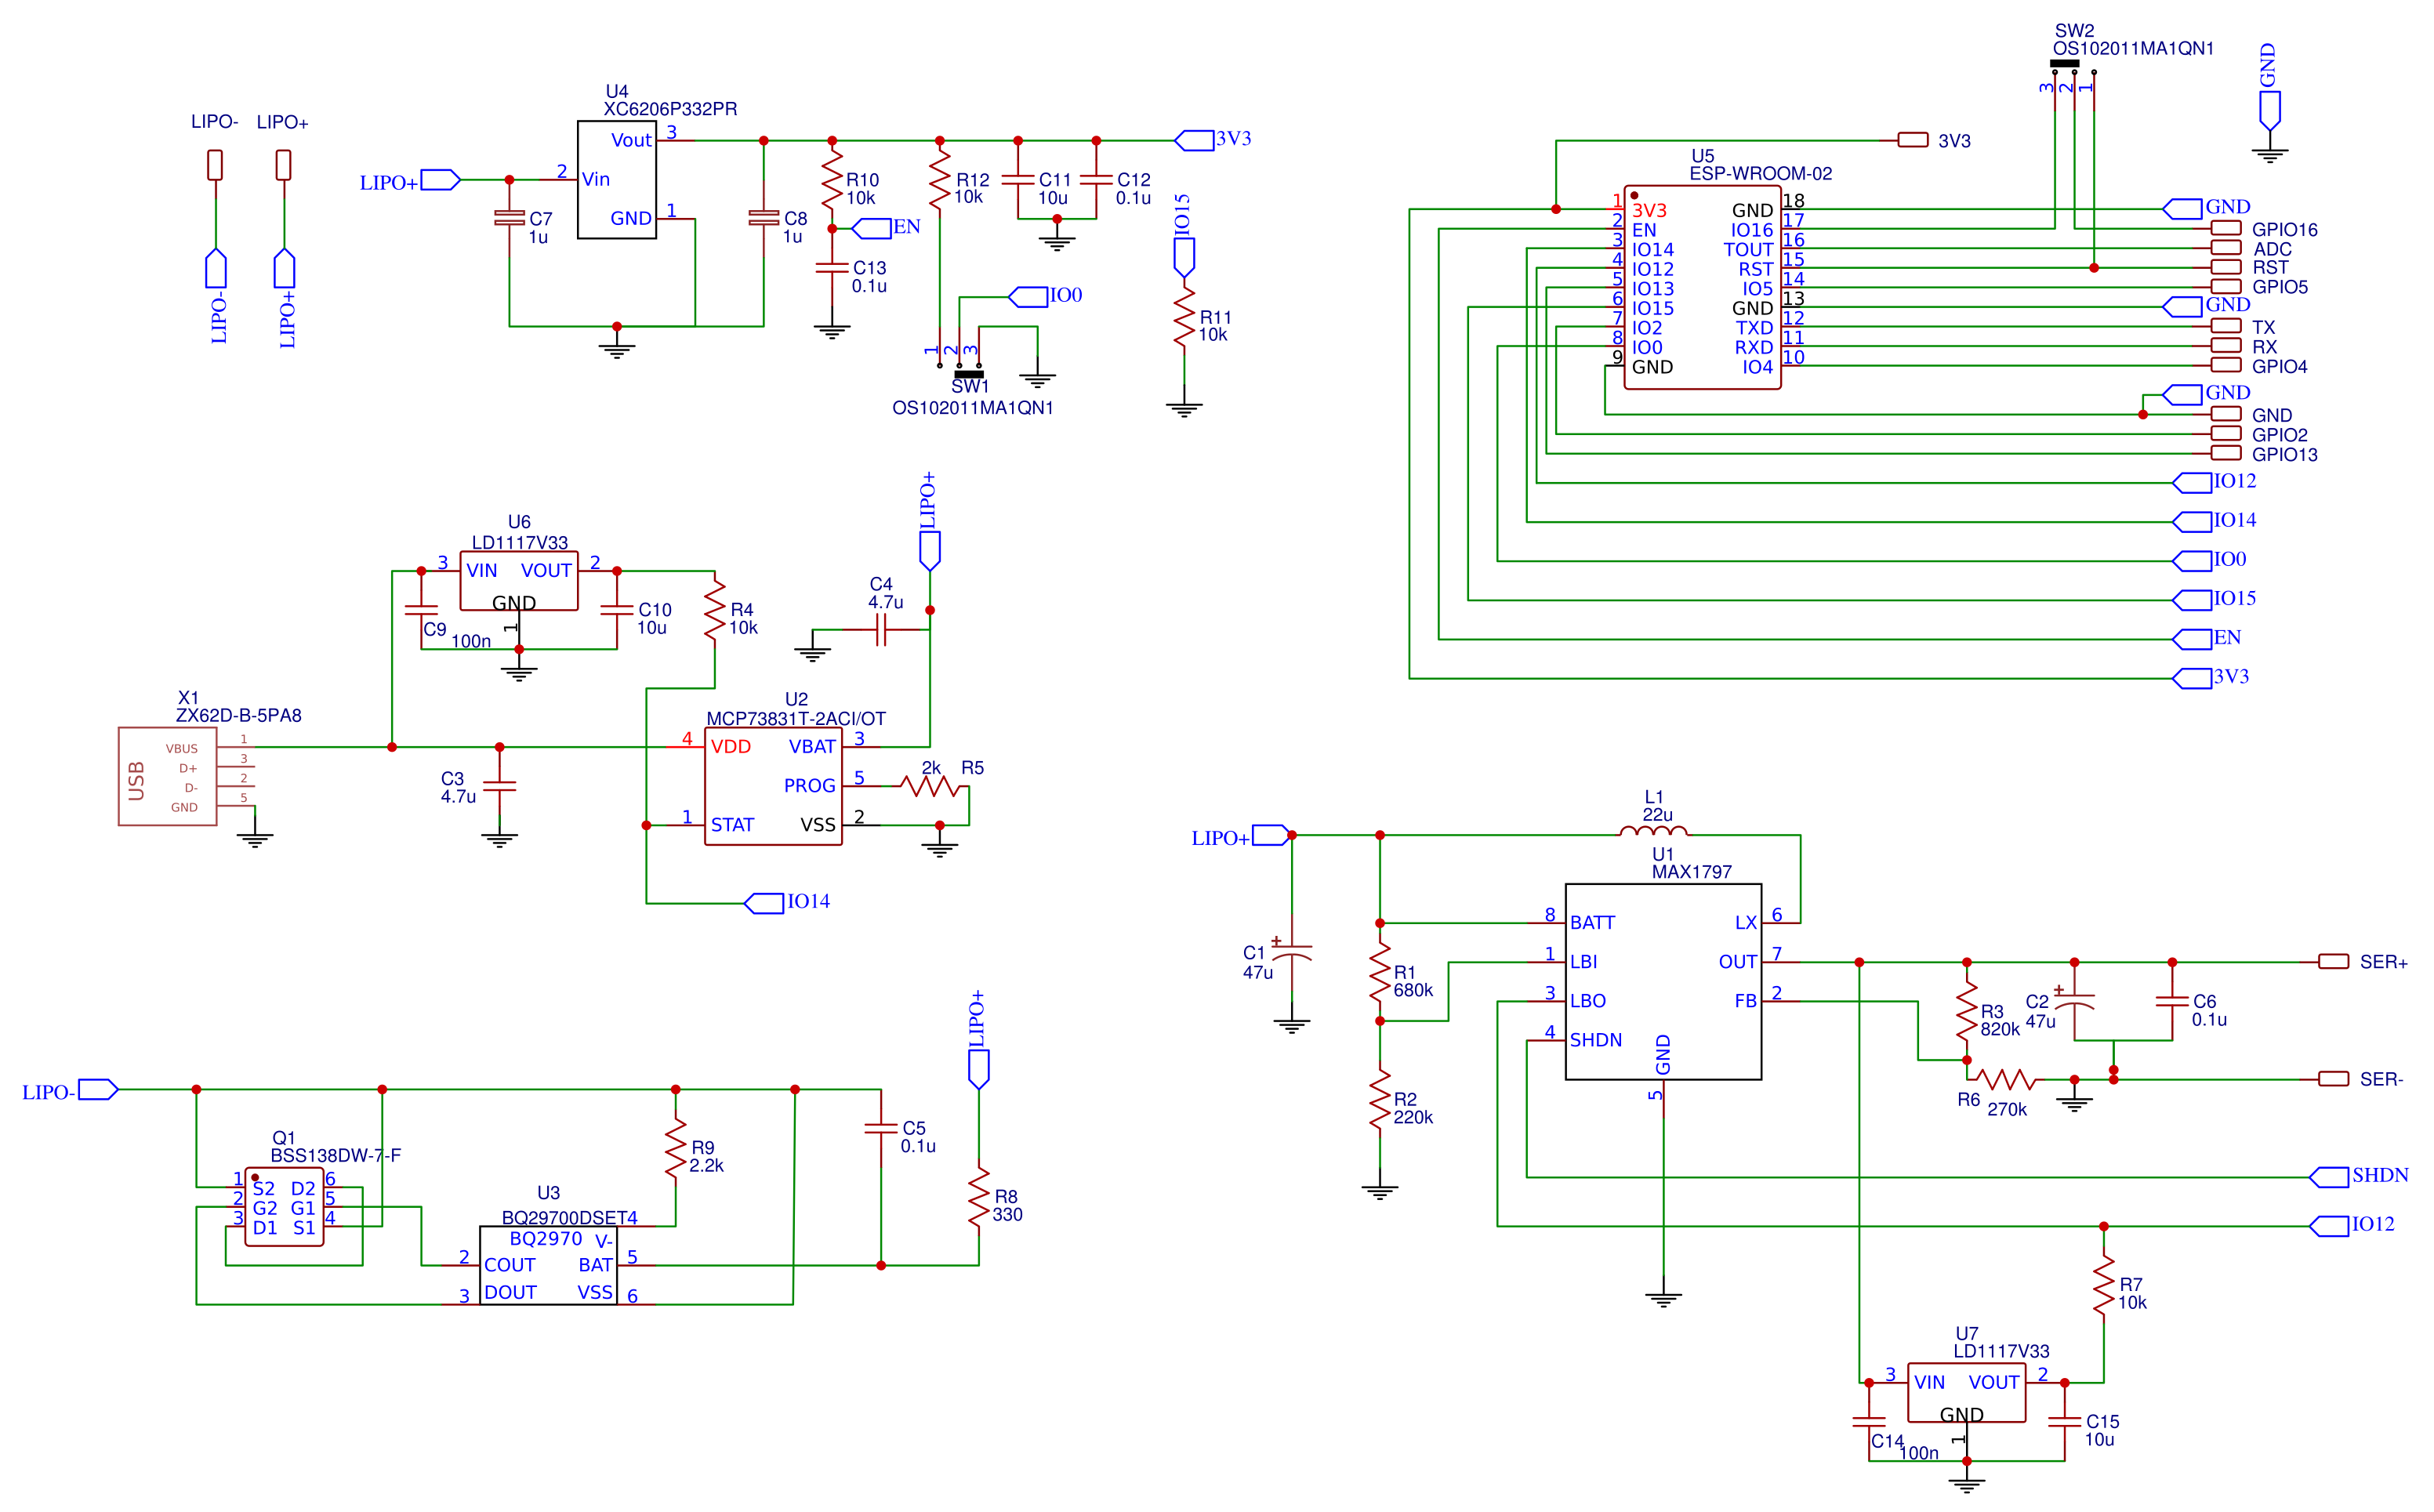
\includegraphics[width=1\textwidth]{images/PCB-sch.png}
               \caption{PCB Schematic}
               \label{fig:pcbsch}
            \end{center}
        \end{figure}
        \newpage
        
        \begin{itemize}
            \item \textbf{U5} - The ESP8266 WiFi module we chose was the ESP-WROOM-02 \cite{esp}:
                \begin{itemize}
                    \item Manufactered by Espressif - the company that makes the internal ESP8266 SoC's, as well as the SDK required to connect the module to Eduroam - we knew it was the safest option in order to connect the system to WiFi. 
                    \item This module has less GPIO pins for our application specific PCB, when comparing it to other solutions such as the ESP-12E WiFi module from AI-Thinker \cite{esp12e}, and hence draws less current.
                \end{itemize}
            \item \textbf{U4} - To convert the 3.7V from the LiPo  to 3.3V for the ESP we used the XC206P332PR \cite{vreg} voltage regulator IC:
            \begin{itemize}
                \item Its a low dropout regulator meaning the ESP would be supplied a stable 3.3V all the time even when the lipo battery was drained.
            \end{itemize}
            \item \textbf{U1} - To convert the 3.7V from the LiPo battery to 5V for the servo we used the MAX1797EUA-T \cite{boostconverter} boost converter IC with a 22uH inductor:
                \begin{itemize}
                    \item With a 2$\mu$A shutdown current and 25$\mu$A quiescent current, when not in use the IC draws little current.
                    \item Its shutdown pin meant we could cut off power to the servo when it was not in use, directly from one of the ESP’s GPIO pins.
                \end{itemize}
            \item \textbf{U2} - To recharge the LiPo battery we used the MCP73831T-2ACI/OT \cite{charge} charging IC.
                \begin{itemize}
                    \item With a charge current of up to 500mA, we could fully charge our LiPo battery in approximately 3 hours.
                \end{itemize}
            \item \textbf{U3} - To make sure the LiPo battery would not overcharge or discharge we used the BQ29700DSET \cite{protection} battery protection IC, with added:
                \begin{itemize}
                    \item Charge overcurrent detection;
                    \item Discharge overcurrent detection;
                    \item Load short-circuit detection.
                \end{itemize}
        \end{itemize}


\subsection{Integration}
{Thanks to the solid system architecture, integrating the different parts was in theory relatively painless: the app would connect to the client server and the robot would then connect to the robot server, allowing for wireless control of the devices. That being said, the team faced several integration issues, which can mostly be summarized as having belonged to one of the following classes:}
    \begin{itemize}
        \item {API Mismatches. Sometimes the server and the application teams would get out sync regarding what the exact behaviour of the different API endpoints were. Initially the team set out to create a complete API specification that would always be kept up to date, but as time went on this became difficult to manage due to last-minute bug fixes.}
        \item {OAuth2.0 issues. While developing the OAuth2.0 authentication mechanism, the team faced a lot of issues integrating the app and the servers; for example, Ory Hydra requires HTTPS for the callback URL, but handling this on Android requires setting up App Links if you want to support newer versions of the operating system.}
        \item {Robot software complications. For example, getting the robots to connect to Eduroam proved a very time-consuming process due to its WPA2-Enterprise protocol; whilst the robots worked well in isolation it was therefore surprisingly difficult to integrate them with the rest of the system.}
    \end{itemize}
\subsection{Testing}
    \subsubsection{Software Testing}
        {Throughout the project we put a lot of emphasis on software testing in order to minimize integration issues. For example, the web server had a separate test and production environment: the test environment was based off the Git \textit{webserver} development branch, whereas the production branch was based off master. This allowed for deploying and testing changes to the web server without interrupting the app development, and instilled confidence in our system. Unfortunately, a lot of the unit tests were removed towards the end of the project; as more and more last-minute changes and refactoring was added to meet the tight deadlines, tests became out of sync with functionality. However, while the number of software tests set up decreased as the project went along, we did make use of continuous integration throughout, so all tests available were run whenever a pull request was opened to make sure that new changes did not break any of the old functionality.}
    \subsubsection{User Testing}
        {To ensure that the app’s user interface was intuitive and appeared professional, we carried out small-scale user testing before the third demonstration on other students in the SDP cohort. Here, the students were instructed to carry out the following tasks using the application interface:}
            \begin{itemize}
                \item Turn the thermostat up
                \item Turn the living room light off
                \item Rename the thermostat
                \item Move the thermostat to the bottom row
                \item Set up a new switch
            \end{itemize}
        {This testing was carried out using mock-ups as the new UI had not yet been implemented; we believe that this limited the usefulness of the data collected, and note that it was done merely out of a lack of time to implement the UI before testing. We delay discussion of the results and consequences of this testing until the next section, Results.}


%% RESULTS %%
\section{Results}

    \subsection{User Testing}
        {Out of the five testers selected, all five managed to achieve the first four tasks without hesitation. Some minor inconsistencies were observed, were some users for example first tried to perform the task using patterns that are commonly seen in iPhone apps but not on Android, but users quickly self-corrected themselves and adapted to the application’s interface. However, users struggled greatly when it came to calibrate the new switch:}
            \begin{itemize}
                \item {4 out of 5 did not read the on-screen instructions}
                \item {4 out of 5 failed to make the connection between what they were inputting on the app and what the robot was doing in the real world}
                \item {All five found the repetitive nature of calibration confusing}
                \item {There was general confusion regarding how the user’s input affected the calibration}
            \end{itemize}
        {As a response to this, we abandoned the proposed method of calibration, where the robot would try different settings and the user would input when it had succeeded. Instead a previous design was implemented, where users would adjust the parameters by setting their values manually through trial-and-error.}
        
    \subsection{Costs}
        {We estimate that producing and supporting a single pair of Bolt-Lock PAL and HAL would cost £20.26 in total. Though this does not include labour or marketing costs, it is noticeably lower than the prices of other similar products discussed in \textit{Background}. Finally, note that most of the cost is due to producing the PCB, which would drop sharply in mass production; JLPCB \cite{jlpcb}, a PCB producer based in China, gave a quote of £0.087 per board when ordering 10000 boards. This price does not include the components on the PCB, however even with components it is reduced tenfold.}
    
         \begin{center}
            \begin{tabular}{||c | c ||} 
                 \hline
                 Component & Cost (£) \\ [0.5ex] 
                 \hline\hline
                 Printed Circuit Board (including components) & 14.67\\ 
                 \hline
                 PLA for 3D-Printing & 5.13\\
                 \hline
                 Server (per user, per year) & 0.46\\
                 \hline\hline
                 Total & 20.26\\
                 \hline
            \end{tabular}
        \end{center}
        
    
    \subsection{Trade Fair}
        {The products worked mostly well throughout the trade fair, which we were happy to see. There were however a few complications; namely some of the PCBs were partially short circuited due to the short amount of time left to solder the PCBs. This meant that we:}
            \begin{itemize}
                \item {Had to partially rely on NodeMCU’s for backup}
                \item {Could not demo the thermostat PAL due to a lack of hardware}
                \item {Did not have time to test the final iteration of the thermostat PAL}
            \end{itemize}
        {Despite this, we believe that we managed to showcase our product’s potential well; the switch and bolt lock PALs worked throughout the day with only minor hiccups, and guests at the fair appeared to enjoy interacting with them through Alexa and the Android app.}


%% DISCUSSION %%
\section{Disscusion}
    \subsection{Lessons Learnt}
        {In this project, we have all come to learn quite a few lessons. The following are the five lessons which come to mind the most when reflecting on our experiences:}
            \begin{itemize}
                \item {Taking the time to sit down and plan the entire system architecture from the start saves a lot of time later on.}
                \item {Even with Gantt charts and proper planning it is hard to accurately estimate how long tasks will take to carry out.}
                \item {Despite being the developer of the system, documenting it concisely and accurately is challenging.}
                \item {Supporting industry standards such as the OAuth2.0 authentication standard is a time-consuming and often surprisingly poorly documented task.}
                \item {Managing seven or eight individuals working on a single project is not easy, especially when it is hard to estimate in advance how motivated each person will be.}
            \end{itemize}
        {As a result, there are a number of things we wish we had done differently:}
            \begin{itemize}
                \item {We should have allocated more resources to 3D-printing.}
                \item {We should have tried to finish the individual components earlier to leave more time for integration.}
                \item {We should have assigned a person to be responsible for report writing and marketing for the product so that these tasks had been assigned more priority.}
                \item {We should have started manufacturing the PCBs earlier to leave more time for soldering and bug fixing.}
            \end{itemize}
        {However, all of these largely boil down to the fact that there was a strong lack of resources available to our team. Though all eight active members of the team were very hard-working, we simply did not have more resources to allocate. Clearly, the real mistake made by our team was that we underestimated how much work this project would take to complete; in our blind pursuit of producing something unique compared to our cohort, we failed to take into account that we would only have about $8 \cdot 200 = 1600$ hours to do so.}
    
    \subsection{Future Work}
    There is a lot of work remaining that could increase the marketability and performance of the product:
    \begin{enumerate}
        \item Adding sensors to the hardware to gather data about the environment, for example to verify that a task was completed successfully.
        \item Using machine learning to predict user behaviour using the sensor data, e.g. learning that a user always turns their light on when the sun starts setting.
        \item Reducing power draw, either by optimizing the hardware components more or improving the amount of time that the chips can spend sleeping, and the depth of that sleep.
        \item Reducing form factor by optimizing the PCB size and minimizing the 3D-printed parts
        \item Developing more PALs to support more use cases.
    \end{enumerate}

%% CONCLUSION %%
\section{Conclusion}

We have developed our range of Smart Home Adapters in order to fill a gap in the smart home market. The adapters offer remote control, either through an Android app or using Alexa voice control, of existing devices such as switches, thermostats, and bolt locks. This remote control is done securely using industry-standard authentication mechanisms, and places minimal computational burden on the user's devices thanks to the cloud-hosted server solution. Compared to the competition, these robotic adapters provide unrivalled flexibility at a potentially smaller price. Nonetheless, much work remains before this product is ready to hit the market. 

%% REFERENCES/BIBLIOGRAPHY %%
\begin{thebibliography}{10}

\bibitem{smarthomemarket}
 Statista: The Statistics Portal,
 "Smart Home Revenue, Worldwide",
  [ONLINE] Available at: \url{https://www.statista.com/outlook/279/100/smart-home/worldwide}. [Accessed 4 April 2019].
  
 \bibitem{homeowners}
   Department for Work and Pensions,
 "Family Resources Survey 2016/2017",
  [ONLINE] Available at: \url{https://assets.publishing.service.gov.uk/government/uploads/system/uploads/attachment_data/file/692771/family-resources-survey-2016-17.pdf}. [Accessed 4 April 2019].
  
  \bibitem{nestprice}
  Nest,
  "Nest Learning Thermostat: Overview",
  [ONLINE] Available at: \url{https://nest.com/uk/thermostats/nest-learning-thermostat/overview/}. [Accessed 4 April 2019].
  
  \bibitem{hiveprice}
  Hive,
  "Hive Active Heating",
  [ONLINE] Available at: \url{https://www.hivehome.com/products/hive-active-heating/buy}. [Accessed 4 April 2019].
  
  \bibitem{hueprice}
  Phillips Hue,
  "Starter kit E27",
   [ONLINE] Available at: \url{https://www2.meethue.com/en-gb/p/hue-white-white-and-color-ambiance-starter-kit-e27/8718696449592}. [Accessed 4 April 2019].
   
   \bibitem{wemoprice}
   Belkin,
   "WeMo Switch",
   [ONLINE] Available at: \url{https://www.belkin.com/uk/p/P-F7C027/}. [Accessed 4 April 2019].
   
   \bibitem{androidmarket}
    Statista: The Statistics Portal,
    "Global market share held by the leading smartphone operating systems in sales to end users from 1st quarter 2009 to 2nd quarter 2018",
     [ONLINE] Available at: \url{https://www.statista.com/statistics/266136/global-market-share-held-by-smartphone-operating-systems/}. [Accessed 8 April 2019].
   
   \bibitem{alexamarket}
   Statista: The Statistics Portal,
   "Worldwide intelligent/digital assistant market share in 2017 and 2020, by product",
    [ONLINE] Available at: \url{https://www.statista.com/statistics/789633/worldwide-digital-assistant-market-share/}. [Accessed 8 April 2019].
    
    \bibitem{androidsdk}
    Android Developers,
    "Command line tools",
     [ONLINE] Available at: \url{https://developer.android.com/studio/command-line/}. [Accessed 8 April 2019].
     
     \bibitem{kotlin}
     Jake Wharton,
     "Using Project Kotlin for Android",
     [ONLINE] Available at: \url{https://docs.google.com/document/d/1ReS3ep-hjxWA8kZi0YqDbEhCqTt29hG8P44aA9W0DM8/edit?hl=en&forcehl=1#heading=h.9gfal5otoz1u}. [Accessed 8 April 2019].
     
     \bibitem{androidactivities}
     Android Developers,
     "Introduction to Activities",
     [ONLINE] Available at: \url{https://developer.android.com/guide/components/activities/intro-activities}. [Accessed 8 April 2019].
     
     \bibitem{appauth}
     OpenID,
     "AppAuth-Android",
     [SOFTWARE] Available at: 
     \url{https://github.com/openid/AppAuth-Android}. [Downloaded 11 March 2019].
     
     \bibitem{zxing}
     JourneyApps,
     "ZXing Android Embedded",
     [SOFTWARE] Available at:
     \url{https://github.com/journeyapps/zxing-android-embedded}.
     [Downloaded 12 February 2019]
     
     \bibitem{retrofit}
     Square,
     "Retrofit: A type-safe HTTP client for Android and Java",
     [SOFTWARE] Available at:
     \url{https://square.github.io/retrofit/}
     [Downloaded 5 February 2019]
     
     \bibitem{builderdesignpattern}
     w3sDesign,
     "Builder: Problem",
     [ONLINE] Available at:
     \url{http://w3sdesign.com/?gr=c02&ugr=proble}
     [Accessed 8 April 2019]
     
     \bibitem{gson}
     Google,
     "Gson",
     [SOFTWARE] Available at:
     \url{https://github.com/google/gson}.
     [Downloaded 5 February 2019]
     
     \bibitem{go}
     Golang,
     "The Go Programming Language",
     [SOFTWARE] Available at:
     \url{https://golang.org}
     [Accessed Jan 23 2019]
     
     \bibitem{gofast}
     Stream,
     "Why we switched from Python to Go",
     [ONLINE] Available at:
     \url{https://getstream.io/blog/switched-python-go/}
     [Accessed 10 April 2019]
     
     \bibitem{goconcurrency}
     Amigo,
     "Why use Golang?",
     [ONLINE] Available at:
     \url{https://amigotechnology.com/why-use-golang/}
     [Accessed 10 April 2019]
     
     \bibitem{oauth}
     Aaron Parecki,
     "OAuth 2.0 Servers",
     [ONLINE] Available at:
     \url{https://www.oauth.com}
     [Accessed 23 February 2019]
     
      \bibitem{docker}
     Docker,
     "Docker: Enterprise Application Container Platform",
     [SOFTWARE] Available at:
     \url{https://www.docker.com}
     [Downloaded 2 February 2019]
     
     \bibitem{circleci}
     CircleCI,
     "Continuous Integration and Delivery - CircleCI",
     [SOFTWARE] Available at:
     \url{https://circleci.com}
     [Downloaded 20 March 2019]
     
     \bibitem{watchtower}
     containrrr,
     "Watchtower: Automatically update running Docker containers",
     [SOFTWARE] Available at:
     \url{https://github.com/containrrr/watchtower}
     [Downloaded 2 February 2019]
   
    \bibitem{servo1}
    \url{https://servodatabase.com/servo/hitec/hs-322hd}. [Accessed 9 April 2019]
    
    \bibitem{servo2}
    \url{https://engineering.tamu.edu/media/4247823/ds-servo-mg90s.pdf} [Accessed 9 April 2019]
    
    \bibitem{servo3}
    \url{https://servodatabase.com/servo/towerpro/mg92b} [Accessed 9 April 2019]
    
    \bibitem{pi2wifi}
    \url{ https://www.instructables.com/id/Access-Eduroam-on-a-Raspberry-Pi-in-Cambridge/}
    
    \bibitem{wpa2}
    WPA2-enterprise + PEAP,
    [ONLINE] Available at:
    \url{https://github.com/esp8266/Arduino/issues/3527}
    [Accessed 10 April 2019]
    
    \bibitem{nonos}
    ESP8266 Non-OS SDK API Reference,
    [DOCUMENTATION] Available at:
    \url{https://www.espressif.com/en/support/download/documents?keys=&field_type_tid\%5B\%5D=14}
    [Downloaded at 16 February 2019]
    
    \bibitem{sdkstart}
    ESP8266 SDK Getting Started Guide, Chapter 4.1.2,
    [ONLINE] Available at:
    \url{https://www.espressif.com/sites/default/files/documentation/2a-esp8266-sdk_getting_started_guide_en.pdf}
    [Accessed 10 April 2019]
    
    \bibitem{espplugin}
    Arduino core for ESP8266 WiFi chip,
    [SOFTWARE] Available at:
    \url{https://github.com/esp8266/Arduino}
    [Downloaded 2 February 2019]
    
    \bibitem{deepsleep}
    [ONLINE] Available at:
    "RUNNING NODEMCU ON A BATTERY: ESP8266 LOW POWER CONSUMPTION REVISITED"
    \url{https://tinker.yeoman.com.au/2016/05/29/running-nodemcu-on-a-battery-esp8266-low-power-consumption-revisited/}
    [Accessed 10 April 2019]
    
    \bibitem{esp}
    ESP-WROOM-02 Datasheet,
    [DATASHEET] Available at:
    \url{https://www.espressif.com/en/products/hardware/esp-wroom-02/resources}
    [Downloaded 12 March 2019]
    
    \bibitem{esp12e}
    ESP-12E WiFi Module Datasheet,
    [ONLINE] Availible at: 
    \url{https://www.kloppenborg.net/images/blog/esp8266/esp8266-esp12e-specs.pdf}
    [Accessed 10 April 2019]
    
    \bibitem{vreg}
    XC6206 Datasheet,
    "Low ESR Cap.Compatible Positive Voltage Regulators"
    [ONLINE] Available at:
    \url{https://www.mouser.co.uk/datasheet/2/268/20001984g-846362.pdf}
    [Accessed 10 April 2019]
    
    \bibitem{boostconverter}
    MAX1795/MAX1796/MAX1797 Datasheet,
    [ONLINE] Available at:
    \url{https://www.mouser.co.uk/datasheet/2/256/MAX1796-1512735.pdf}
    [Accessed 10 April 2019]
    
    \bibitem{charge}
    MCP73831/2 Datasheet,
    "Miniature Single-Cell, Fully Integrated Li-Ion,
Li-Polymer Charge Management Controllers"
    [ONLINE] Available at:
    \url{https://www.mouser.co.uk/datasheet/2/268/20001984g-846362.pdf}
    
    
    \bibitem{protection}
    BQ2970/BQ2971/BQ2972/BQ2973 Datasheet,
    "bq297xx Cost-Effective Voltage and Current Protection Integrated Circuit for Single-Cell
Li-Ion and Li-Polymer Batteries",
    [ONLINE] Available at:
    \url{http://www.ti.com/lit/ds/symlink/bq2970.pdf}
    [Accessed 10 April 2019]
    
    \bibitem{jlpcb}
    JLPCB Quote,
    [ONLINE] Available at:
    \url{https://jlcpcb.com/quote}
    [Accessed 10 April 2019]
    
\end{thebibliography}


\end{document}
